%This is the first chapter of the dissertation

%The following command starts your chapter. If you want different titles used in your ToC and at the top of the page throughout the chapter, you can specify those values here. Since Columbia doesn't want extra information in the headers and footers, the "Top of Page Title" value won't actually appear.

\chapter[Results][Top of Page Title]{Title of Chapter 1}

This chapter presents the results of the analysis presented in the previous chapter.
We present the full set of signal region distributions after applying the $\mu$ factors derived from the fitting procedure.
We also present the systematic uncertainties in each signal region properly accounting for the correlations of the uncertainties.
As no excess is observed, we show exclusion limits in the sparticle-\lsp plane based on the results of the model-dependent fits and present the model-independent limits.

\section{Signal region distributions}

In \ref{fig:srs_scale,fig:srg_scale,fig:src_scale}, we can see the unblinded distributions of the last scale cut used for each signal region.
These distributions include the $\mu$ scale factors as well as the systematic uncertainties after the fitting procedure.
Each plot shows the distribution from a signal model which is targetted by the given signal region.

These distributions have all cuts applied except for the cut on this scale variable, which allows us to see the additional discrimination provided by the given variable.
Since signal regions with the same numeral have identical cuts on all cuts other than the main scale variable, we show (a) and (b) on the same figure.
The left-most (right-most) arrow shown is the location of the a (b) cut applied in the analysis.
We call these plot \textit{$N-1$} plots, where $N$ refers to the number of cuts applied in the analysis.
The full set of $N-1$ plots in the signal regions for the other variables used in the analysis are shown in \ref{app:n-1_plots}.

A figure showing a summary of the pulls in all of the SRs is shown in \ref{fig:sr_summary}.
This figure shows the integrated data and simulation values above the cut values in the N-1 plots, with the corresponding statistical and systematic uncertainties, for all signal regions simulatneously.
The systematic uncertainties will be discussed in the next section.
From this plot, we can see there is no significant excess of events over the Standard Model background.

This information is also presented in \ref{tab:p0_UL_RJR}.
The table includes the expectations from simulation before applying the $\mu$ scaling factor.
SRG3b shows a small excess, but this is not significant.

In this case, we set both simplified model-dependent limits and model-independent limits on the possible cross-sections from BSM physics.
We first consider the final values of the systematic uncertainties.

\begin{figure}[tbp]
\begin{center}
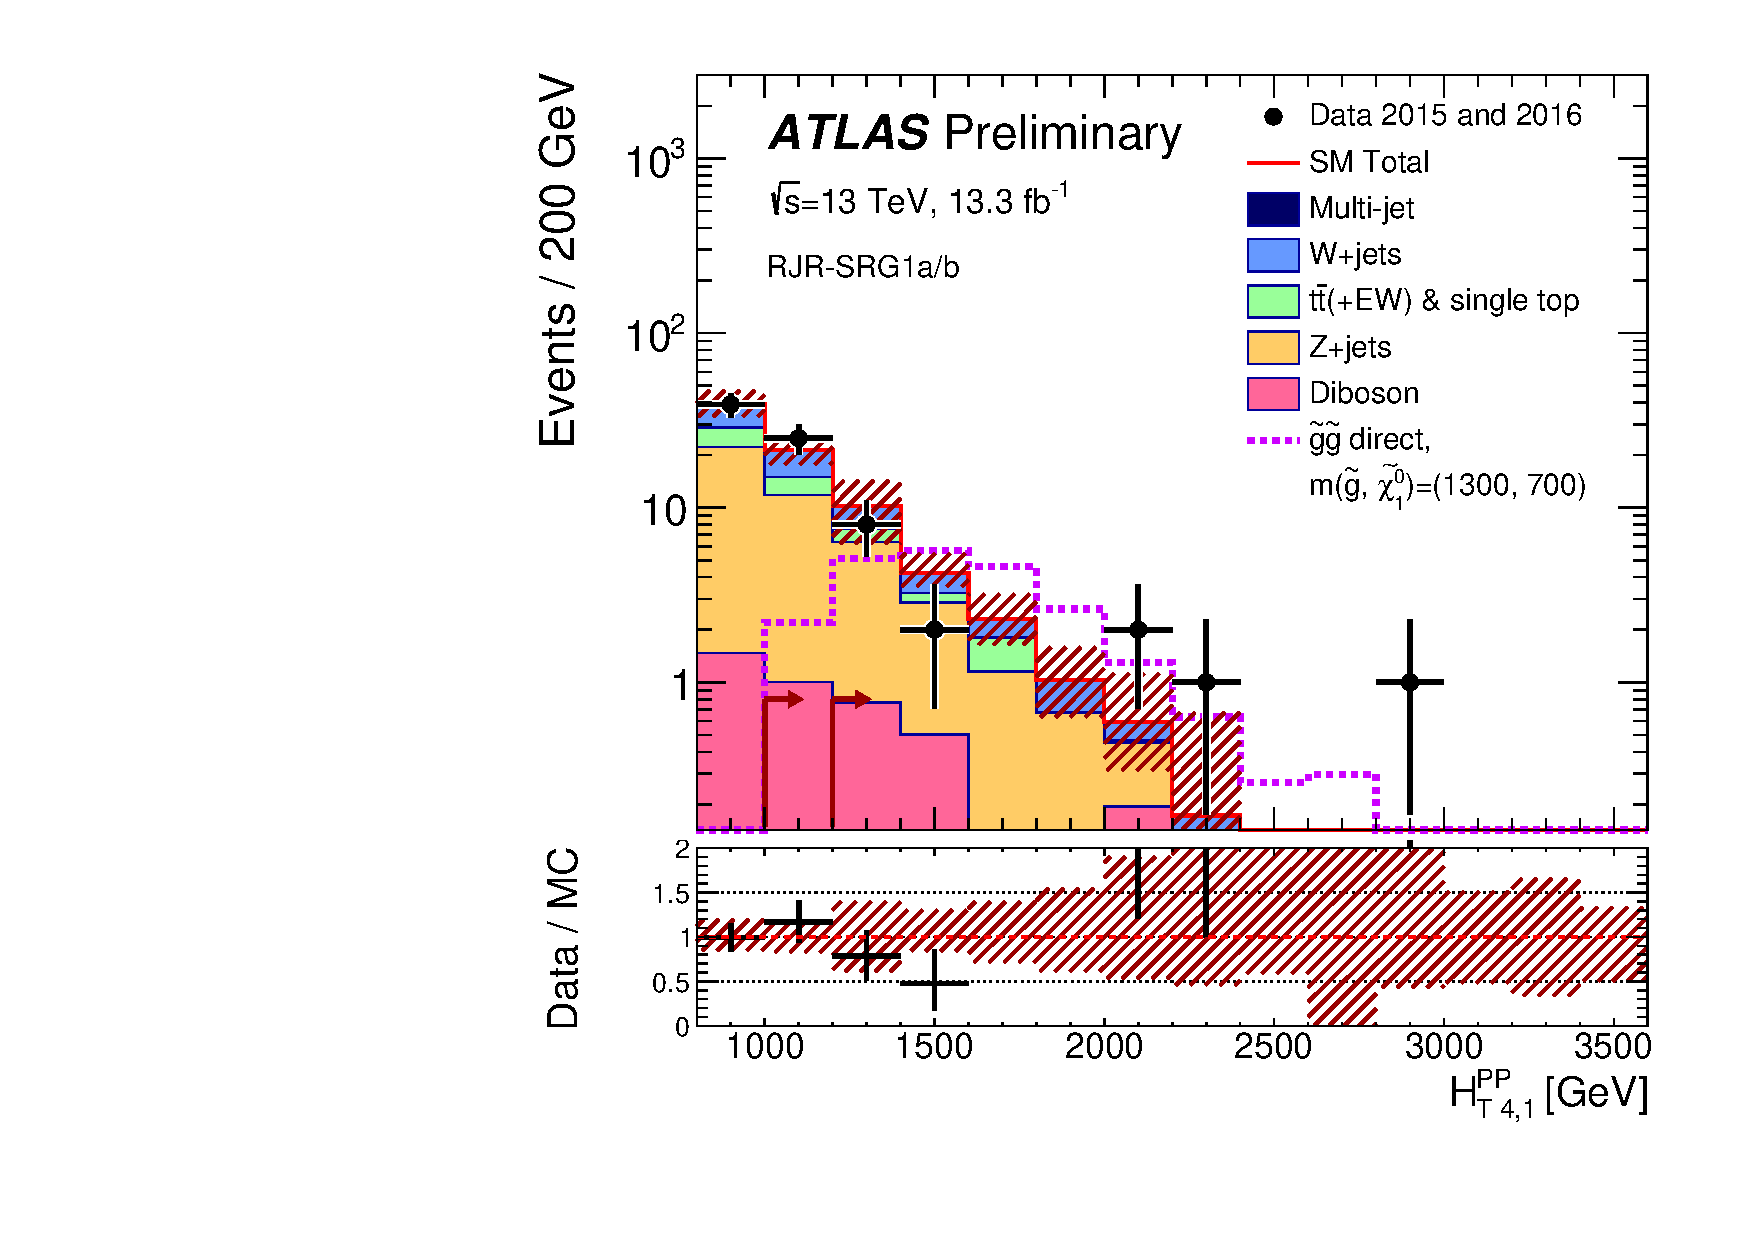
\includegraphics[width=0.45\textwidth]{ATLAS-CONF-2016-078_INT/N-1Plots/AtlasStyle/Preliminary/SR_SRJigsawSRG1a_LastCut_SR_minusone}
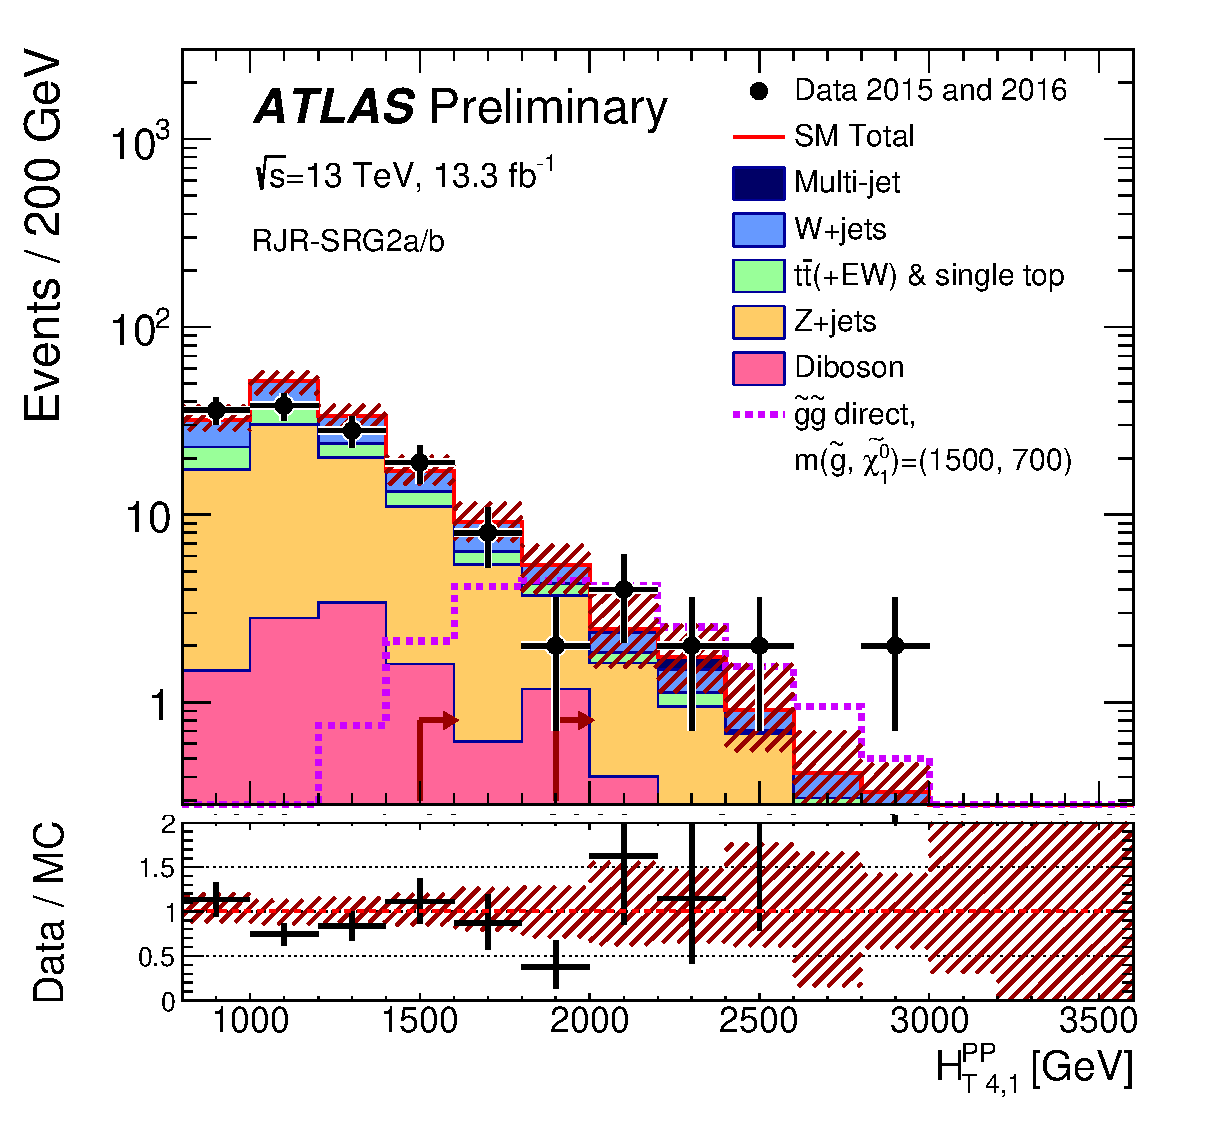
\includegraphics[width=0.45\textwidth]{ATLAS-CONF-2016-078_INT/N-1Plots/AtlasStyle/Preliminary/SR_SRJigsawSRG2a_LastCut_SR_minusone}
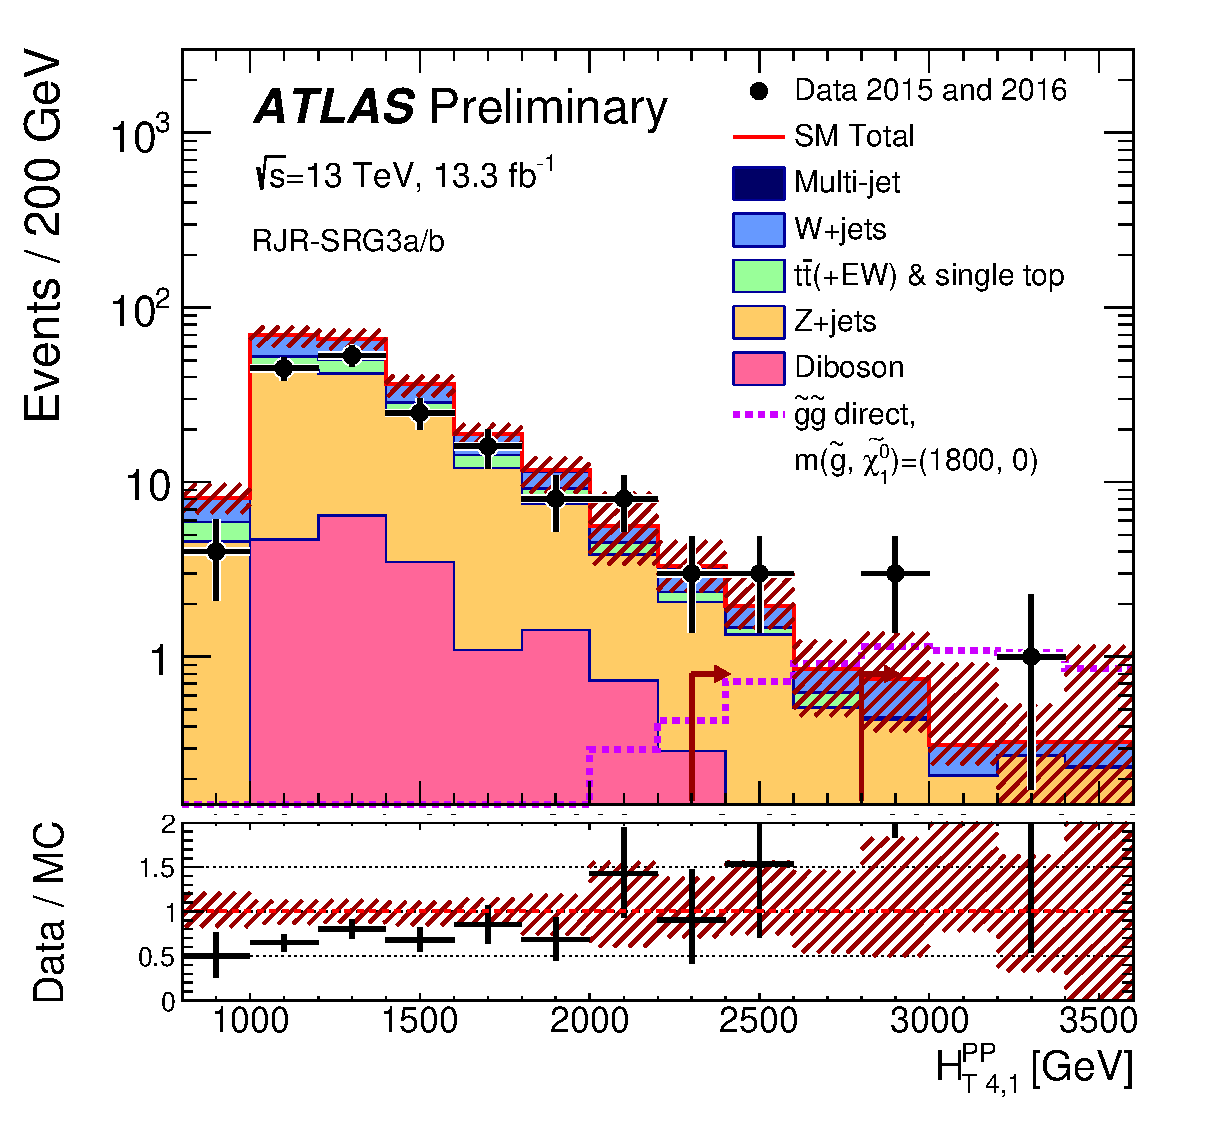
\includegraphics[width=0.45\textwidth]{ATLAS-CONF-2016-078_INT/N-1Plots/AtlasStyle/Preliminary/SR_SRJigsawSRG3a_LastCut_SR_minusone}
\end{center}
\caption{Scale variable distributions for the gluino signal regions.}
\label{fig:srg_scale}
\end{figure}

\begin{figure}[tbp]
\begin{center}
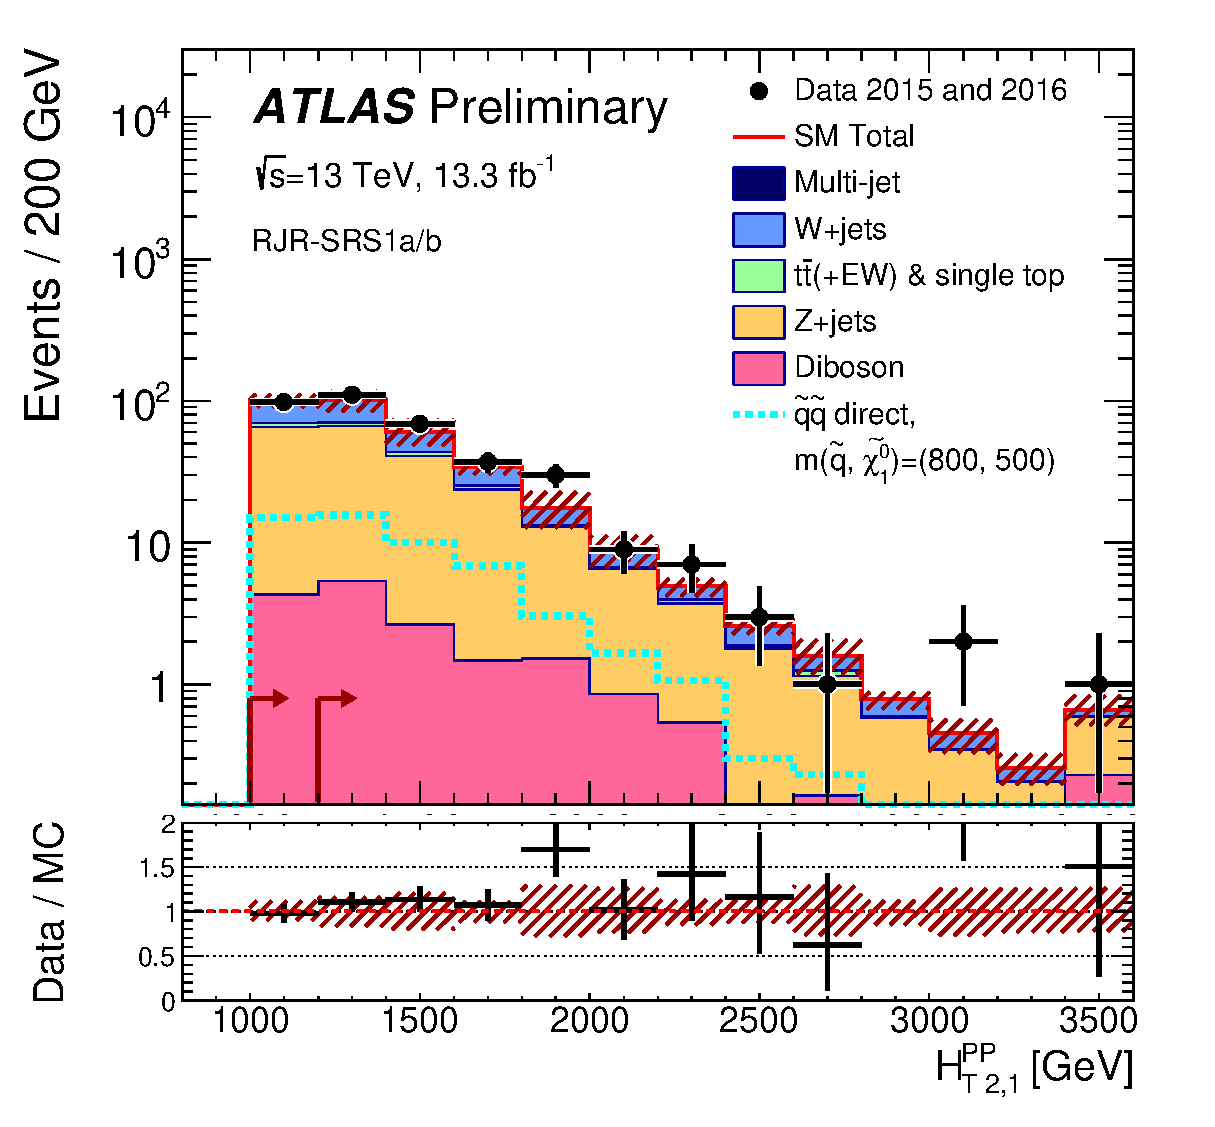
\includegraphics[width=0.45\textwidth]{ATLAS-CONF-2016-078_INT/N-1Plots/AtlasStyle/Preliminary/SR_SRJigsawSRS1a_LastCut_SR_minusone}
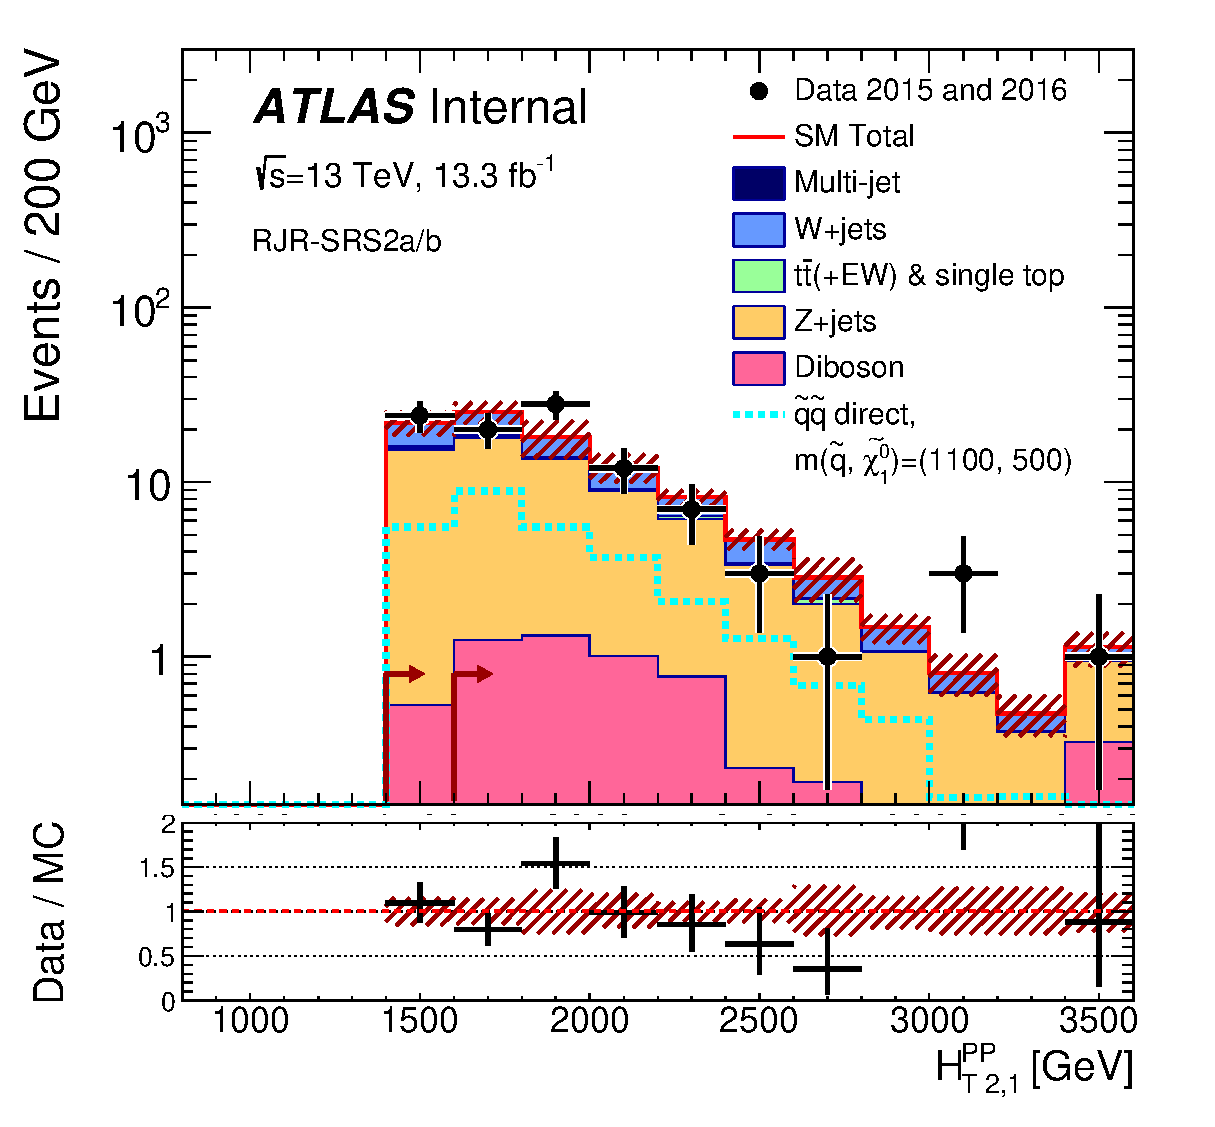
\includegraphics[width=0.45\textwidth]{ATLAS-CONF-2016-078_INT/N-1Plots/AtlasStyle/Preliminary/SR_SRJigsawSRS2a_LastCut_SR_minusone}
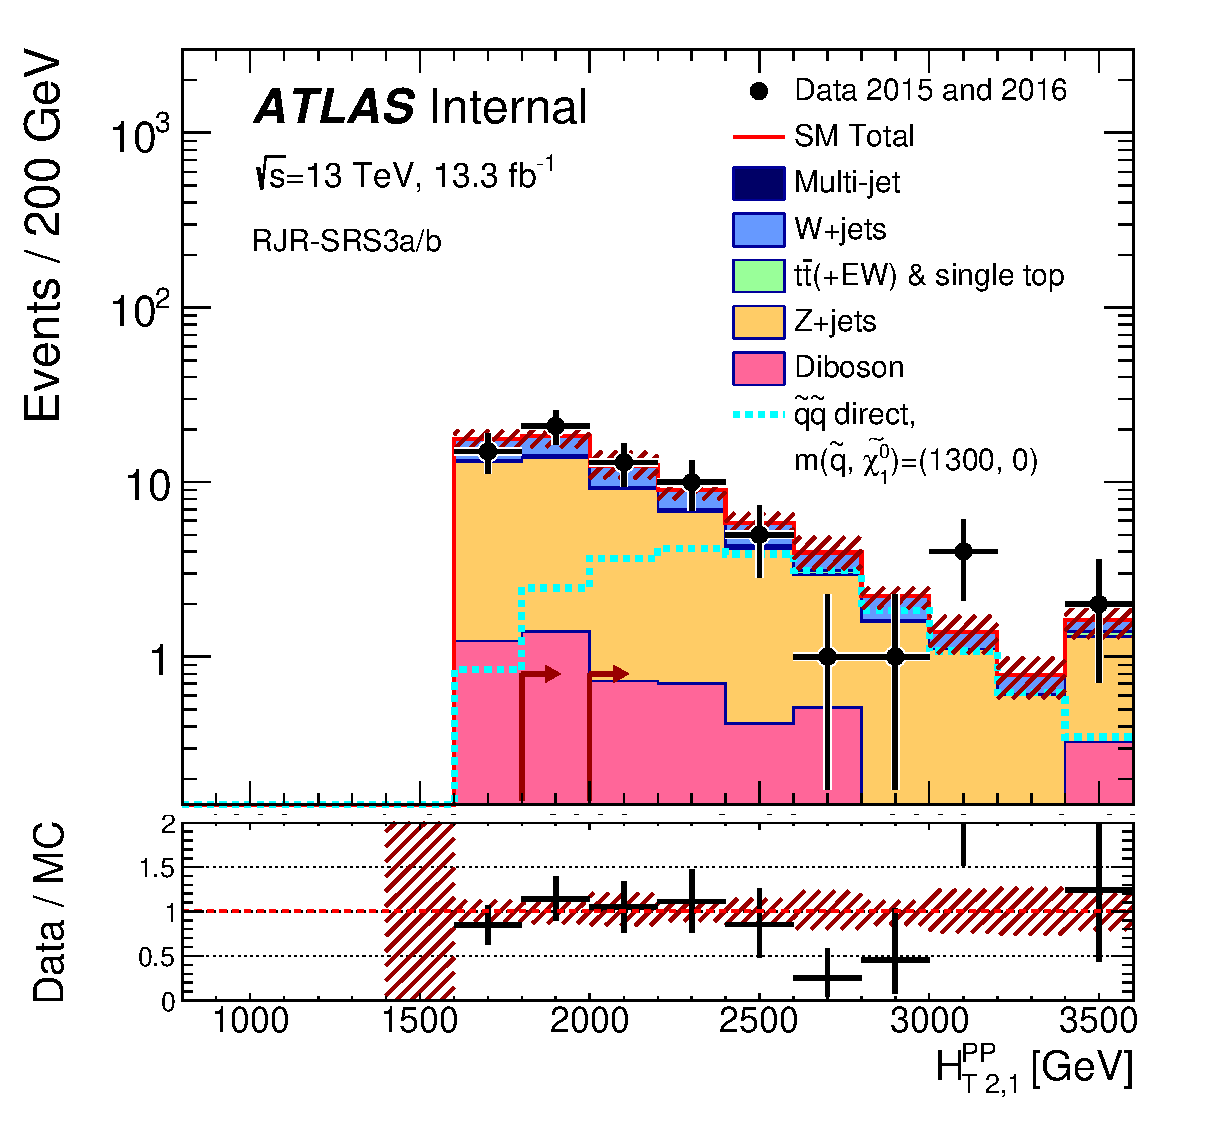
\includegraphics[width=0.45\textwidth]{ATLAS-CONF-2016-078_INT/N-1Plots/AtlasStyle/Preliminary/SR_SRJigsawSRS3a_LastCut_SR_minusone}
\end{center}
\caption{Scale variable distributions for the squark signal regions.}
\label{fig:srs_scale}
\end{figure}

\begin{figure}[tbp]
\begin{center}
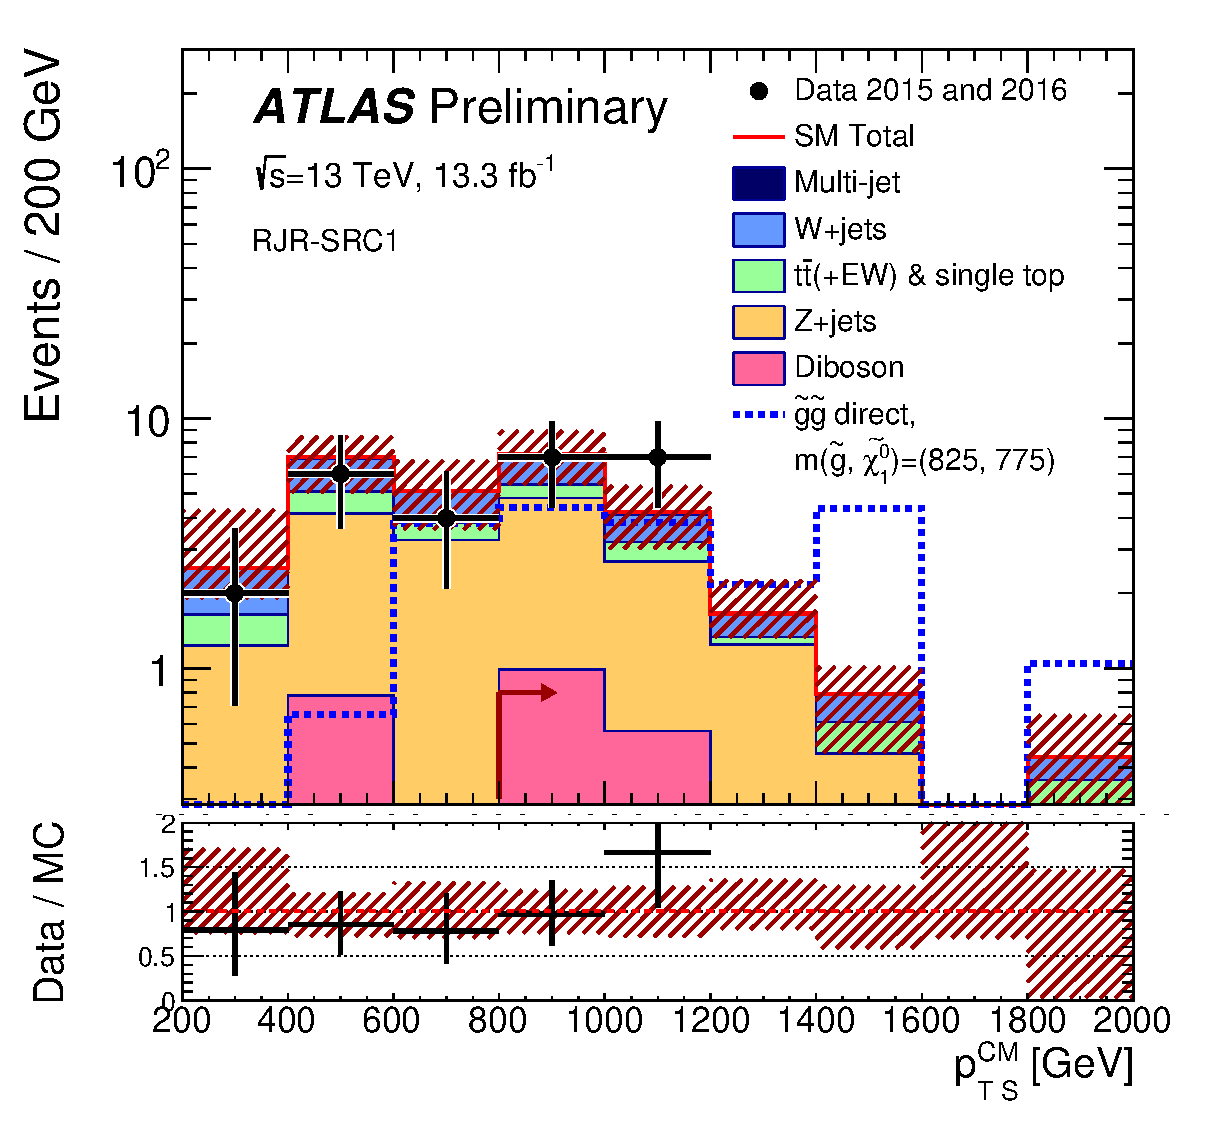
\includegraphics[width=0.45\textwidth]{ATLAS-CONF-2016-078_INT/N-1Plots/AtlasStyle/Preliminary/SR_SRJigsawSRC1_LastCut_SR_minusone}
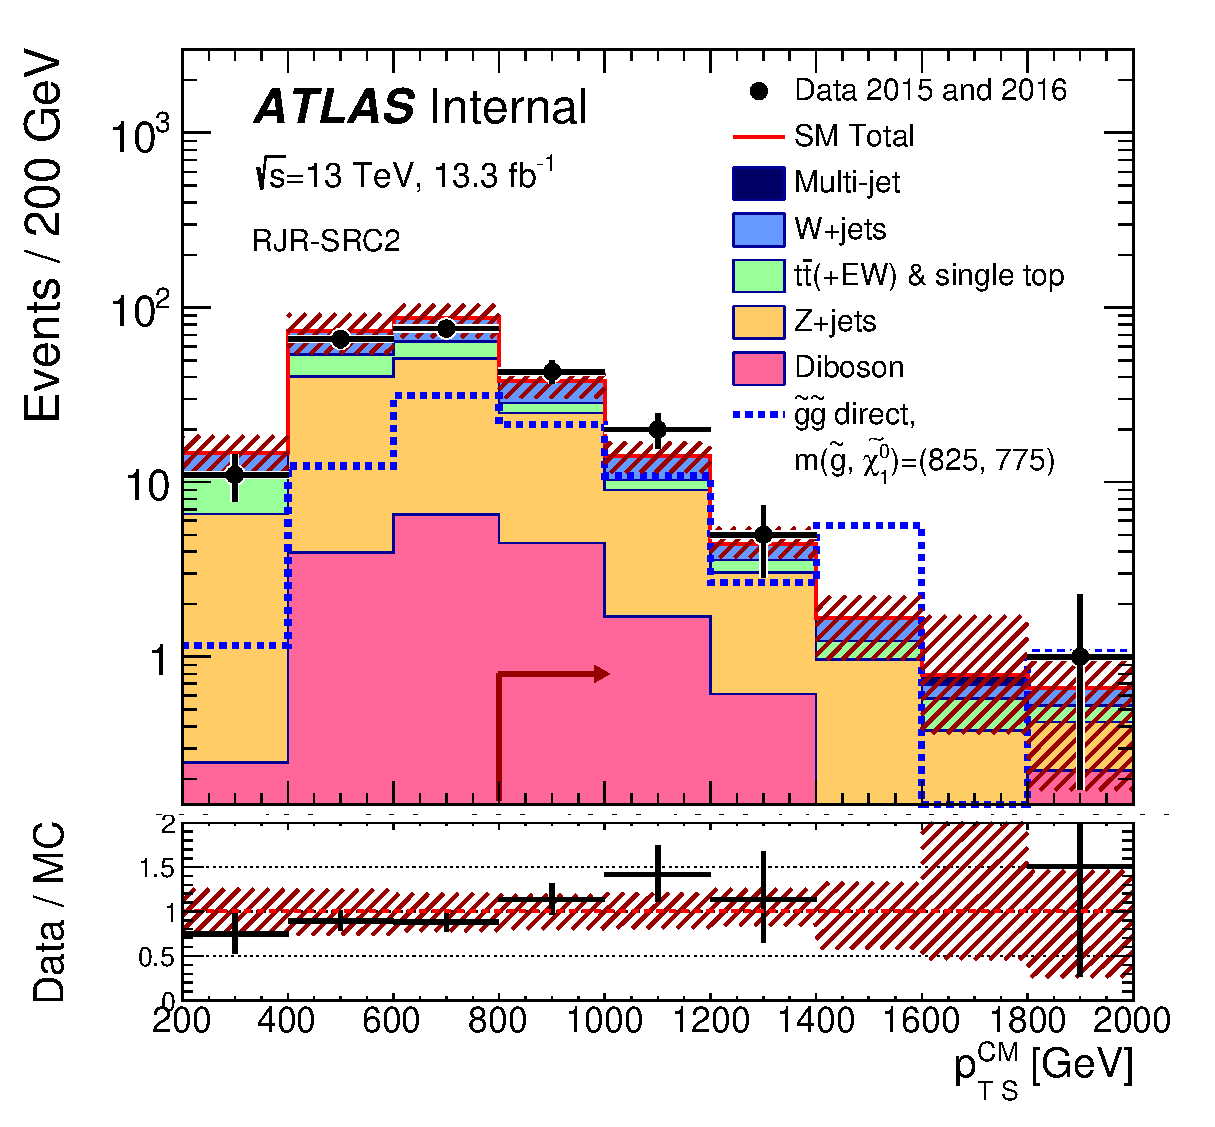
\includegraphics[width=0.45\textwidth]{ATLAS-CONF-2016-078_INT/N-1Plots/AtlasStyle/Preliminary/SR_SRJigsawSRC2_LastCut_SR_minusone}
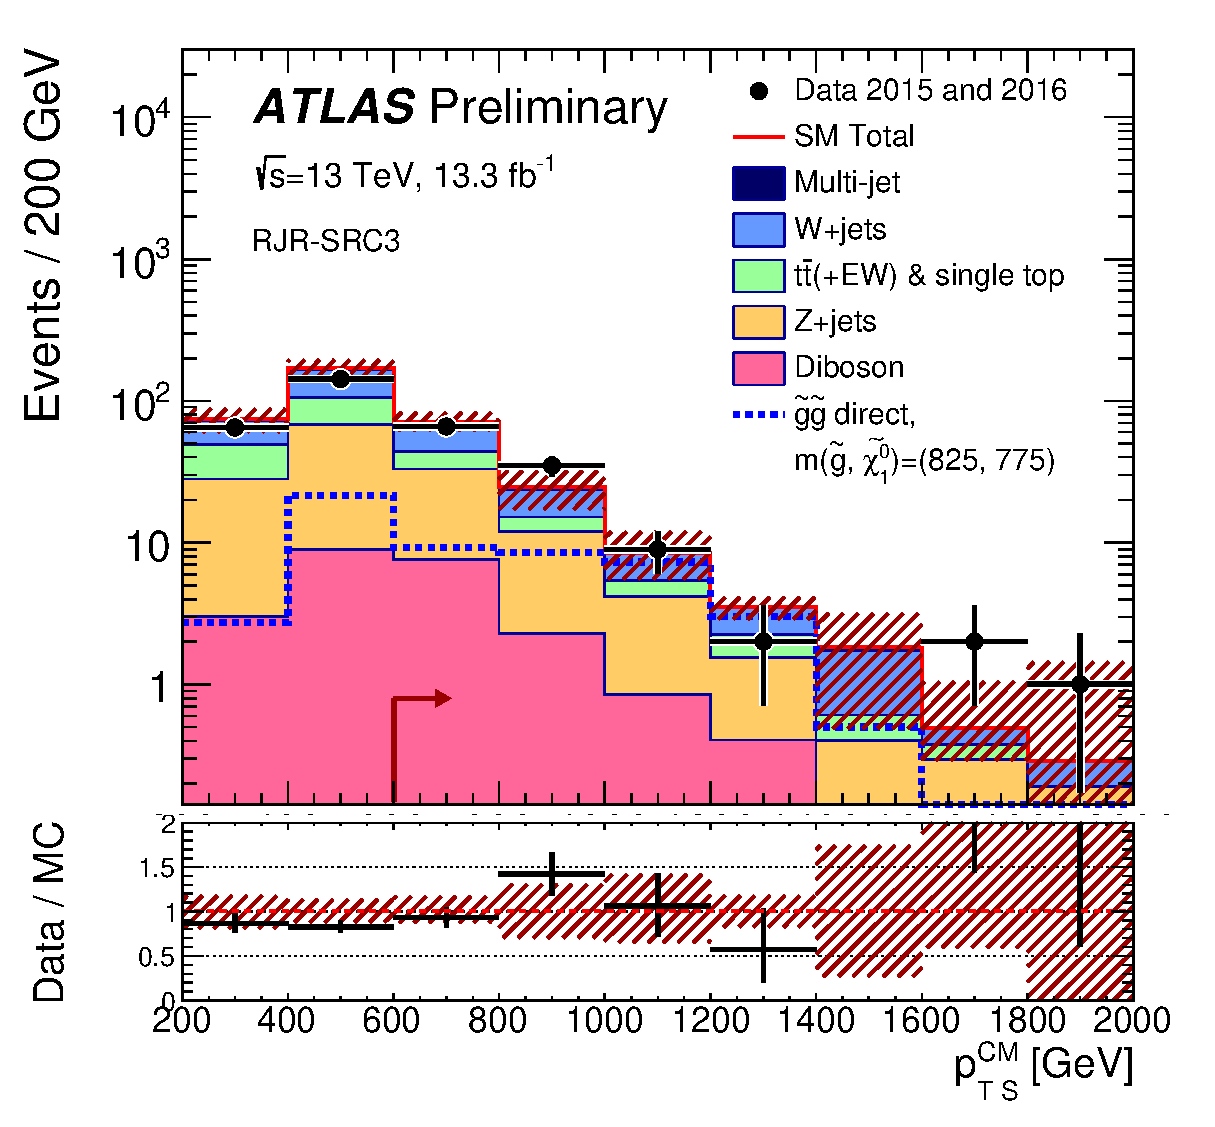
\includegraphics[width=0.45\textwidth]{ATLAS-CONF-2016-078_INT/N-1Plots/AtlasStyle/Preliminary/SR_SRJigsawSRC3_LastCut_SR_minusone}
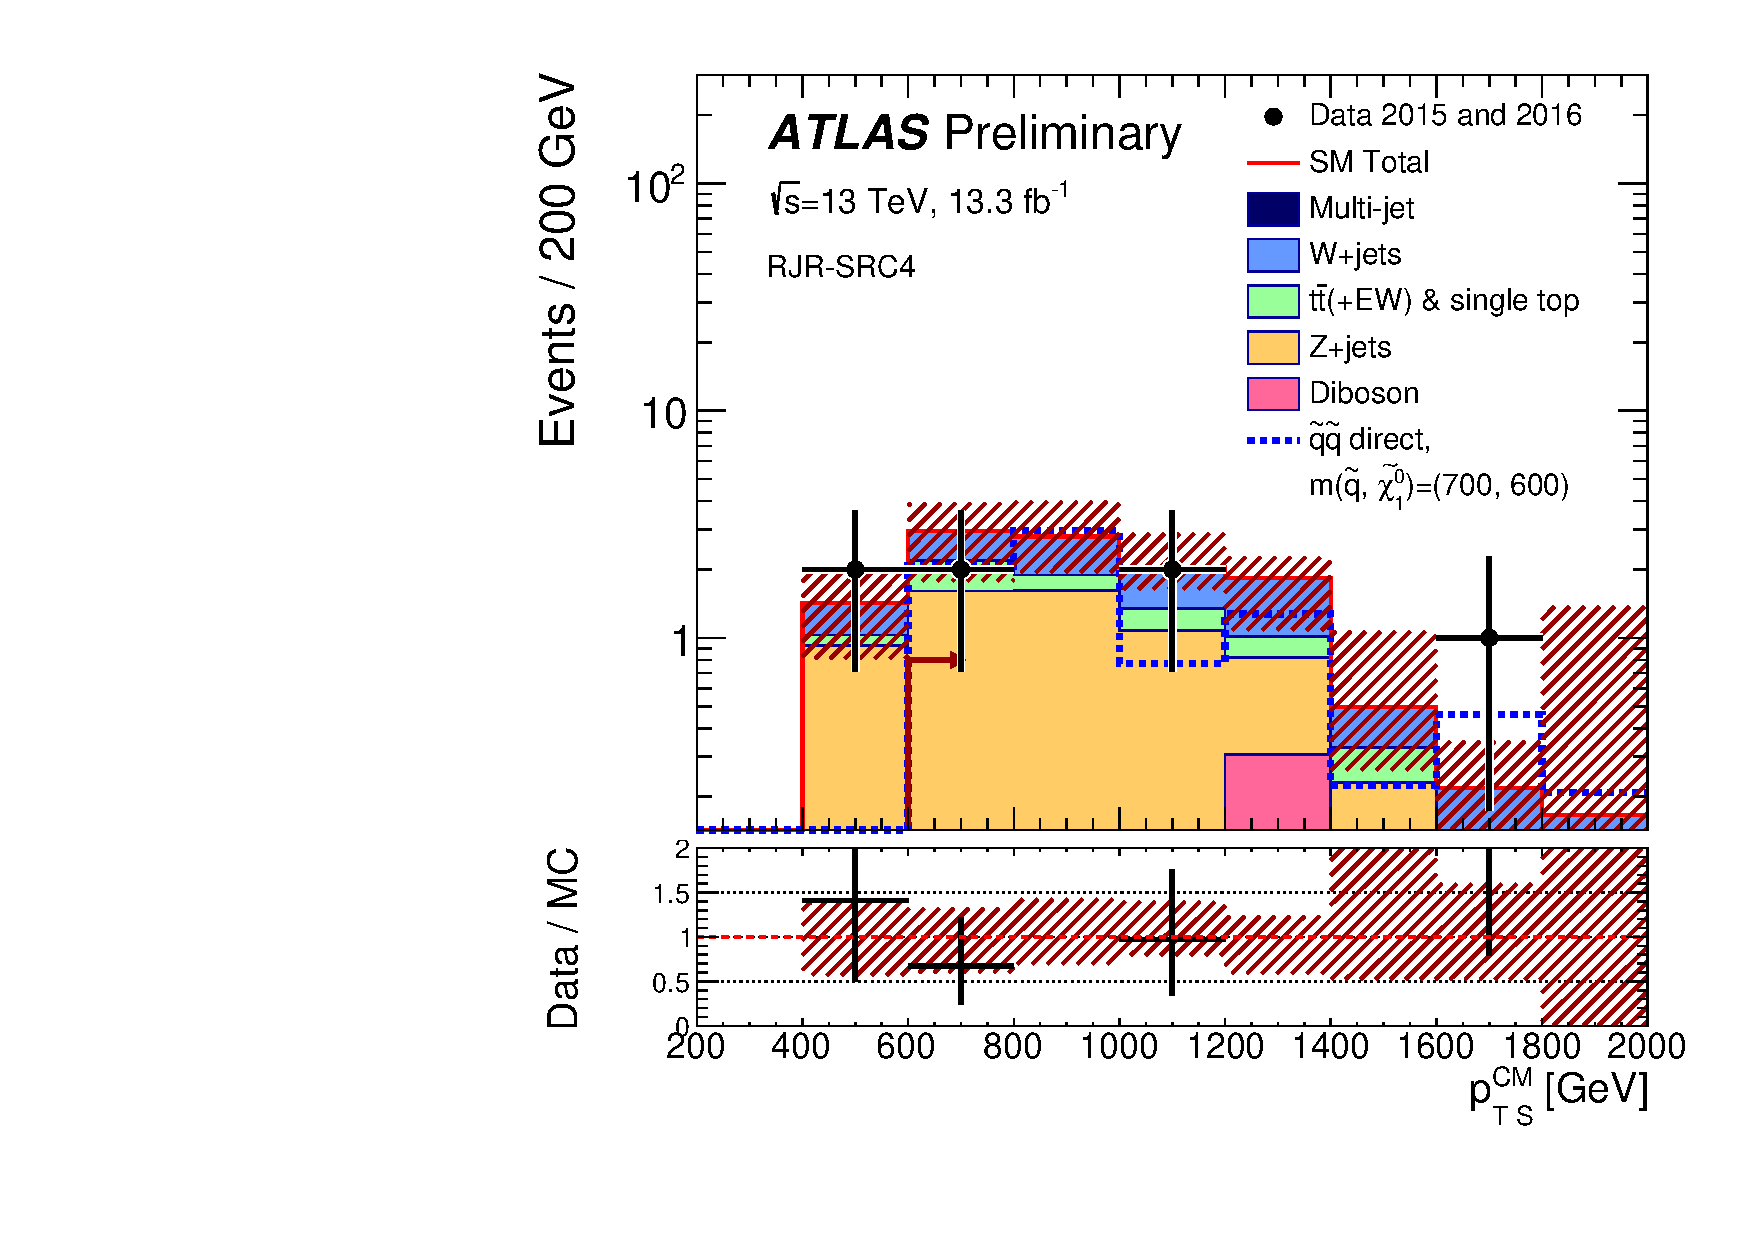
\includegraphics[width=0.45\textwidth]{ATLAS-CONF-2016-078_INT/N-1Plots/AtlasStyle/Preliminary/SR_SRJigsawSRC4_LastCut_SR_minusone}
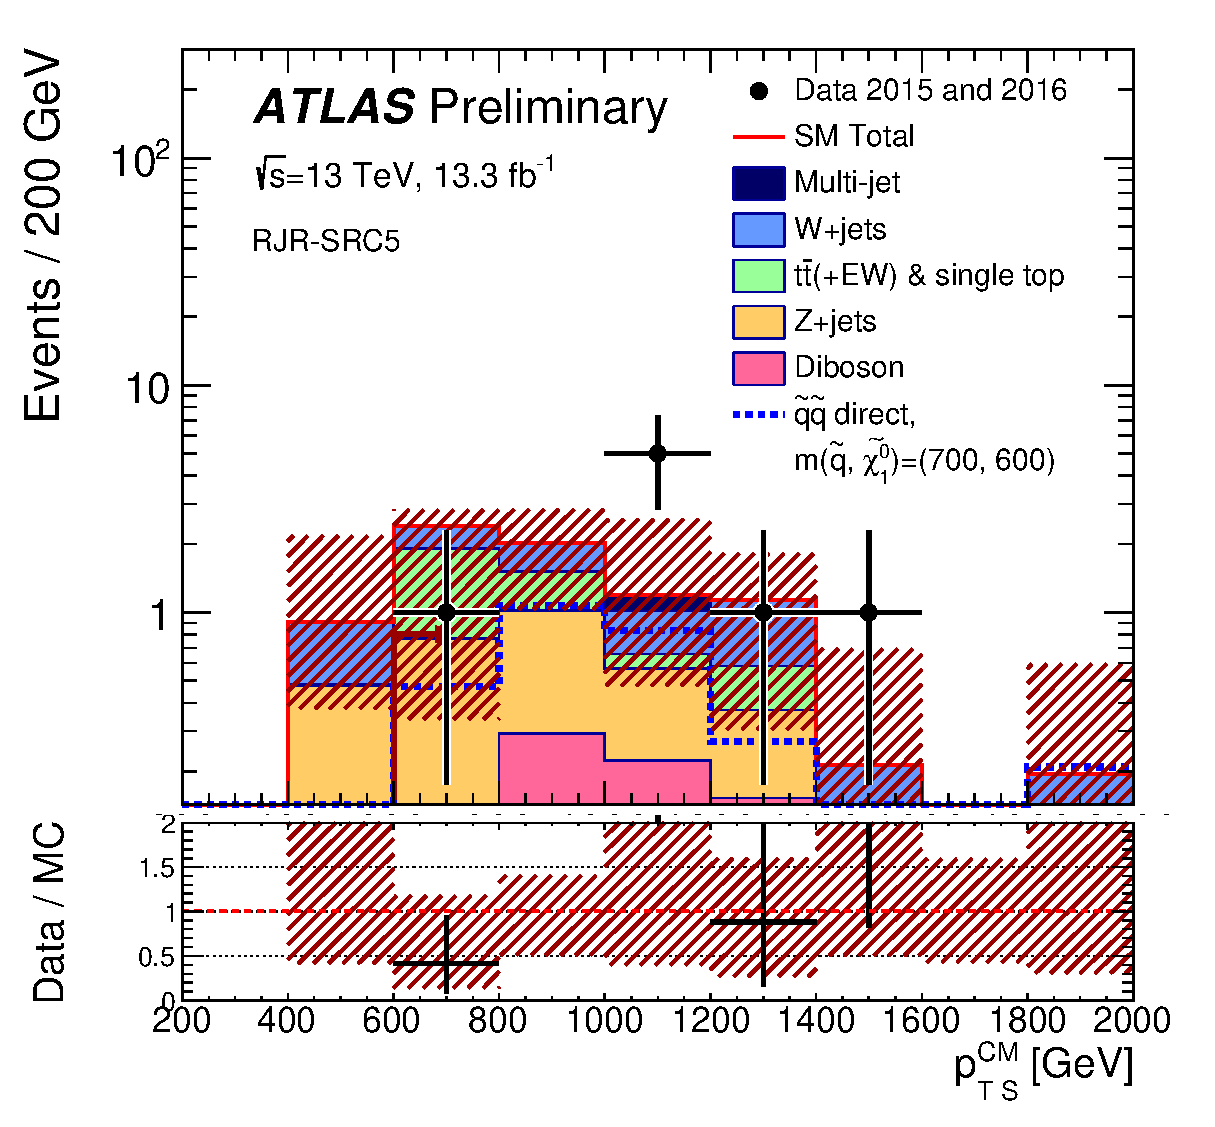
\includegraphics[width=0.45\textwidth]{ATLAS-CONF-2016-078_INT/N-1Plots/AtlasStyle/Preliminary/SR_SRJigsawSRC5_LastCut_SR_minusone}
\end{center}
\caption{Scale variable distributions for the compressed signal regions.}
\label{fig:src_scale}
\end{figure}

\begin{figure}[tbph]
\centering
\caption{Summary of the signal region pulls} \label{fig:sr_summary}
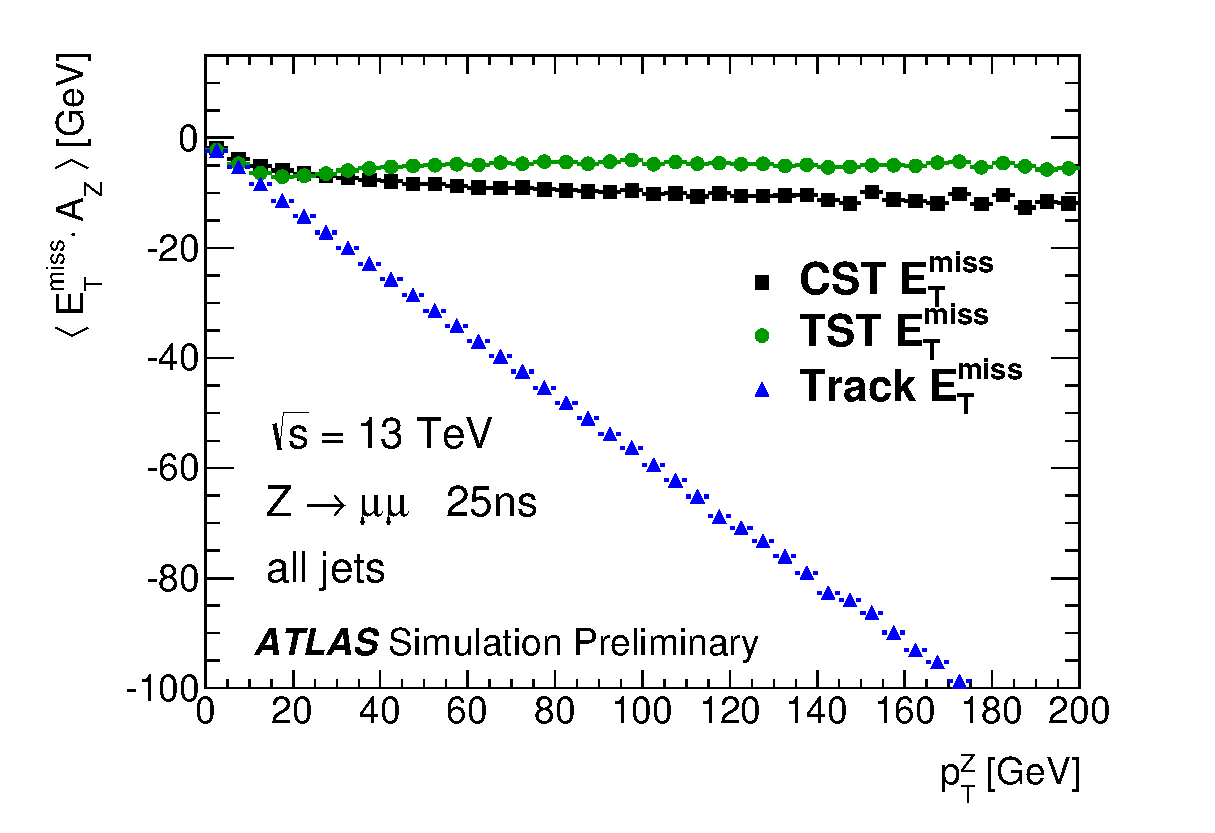
\includegraphics[width=.9\linewidth]{ATLAS-CONF-2016-078/fig_06b}
\end{figure}
\begin{table}[tbp]
\tiny
%\small
\begin{center}
\vspace*{-0.035\textwidth}
\begin{tabular}{|lrrrrrr|}
\hline
Signal Region & \textbf{ S1a } & \textbf{ S1b } & \textbf{ S2a } & \textbf{ S2b } & \textbf{ S3a } & \textbf{ S3b } \\
\hline
\multicolumn{7}{|c|}{MC expected events} \\ \hline
Diboson &  $17$               &  $13$               &  $5.6$               &  $5.1$               &  $4.2$               &  $2.8$               \\
$\mathrm{Z/\gamma^{*}}$+jets &  $231$               &  $163$               &  $63$               &  $48$               &  $36$               &  $24$               \\
W+jets &  $97$               &  $66$               &  $22$               &  $16$               &  $11$               &  $7.8$               \\
$\ttbar$(+EW) + single top &  $15$               &  $10$               &  $2.9$               &  $2.1$               &  $1.7$               &  $1.1$               \\
%%Multi-jet &  $0.93$               &  $0.53$               &  $0.13$               &  $0.00$               &  $0.00$               &  $0.00$               \\
\hline
\multicolumn{7}{|c|}{Fitted background events} \\ \hline
Diboson & $17 \pm 9$ & $13 \pm 7$ & $5.6 \pm 2.8$ & $5.1 \pm 2.6$ & $4.2 \pm 2.1$ & $2.8 \pm 1.4$ \\
$\mathrm{Z/\gamma^{*}}$+jets & $207 \pm 33$ & $146 \pm 23$ & $65 \pm 9$ & $50 \pm 7$ & $37 \pm 5$ & $25.0 \pm 3.5$ \\
W+jets & $95 \pm 9$ & $65 \pm 7$ & $24.1 \pm 2.9$ & $18.3 \pm 2.3$ & $12.8 \pm 2.8$ & $8.7 \pm 2.0$ \\
$\ttbar$(+EW) + single top & $14 \pm 7$ & $9 \pm 5$ & $2.1 \pm 1.7$ & $1.6 \pm 1.3$ & $1.3 \pm 1.0$ & $0.8 \pm 0.7$ \\
Multi-jet &  $0.71_{-0.71}^{+0.71}$               &  $0.41_{-0.41}^{+0.41}$               &  $0.08_{-0.08}^{+0.09}$               & -- & -- & -- \\
\hline
Total Expected MC &  $362$               &  $253$               &  $93$               &  $72$               &  $53$               &  $36$               \\
\hline
Total Fitted bkg & $334 \pm 35$ & $233 \pm 25$ & $96 \pm 10$ & $75 \pm 8$ & $56 \pm 6$ & $37 \pm 4$ \\
\hline
Observed &  $368$                     &  $270$                     &  $99$                     &  $75$                     &  $57$                     &  $36$                     \\
\hline


$\langle\epsilon\mathrm{ \sigma}\rangle_\mathrm{ obs}^{95}$ [fb]   &$7.6$  & $6.5$  & $2.2$  & $1.7$ & $1.6$ & $1.1$ \\
$S_\mathrm{ obs}^{95}$     & $101$ & $86$ & $29$ &  $23$ & $22$ & $15$ \\
$S_\mathrm{ exp}^{95}$     & $ { 78 }^{ +27 }_{ -21 }$ & $ { 61 }^{ +22 }_{ -16 }$ & $ { 28 }^{ +11 }_{ -8 }$ & $ { 23}^{ +9}_{ -7 }$ & $ { 20 }^{ +8 }_{ -6 }$ & $ { 16 }^{ +7 }_{ -5 }$  \\
$p_{0}$ ($\mathrm{Z}$)        & $ 0.20$~$(0.84)$ & $ 0.12$~$(1.17)$ & $ 0.44$~$(0.15)$& $ 0.50$~$(0.00)$ &  $ 0.44$~$(0.14)$ &  $ 0.50$~$(0.00)$ \\
\hline
\end{tabular}

% SRJigsawSRS1a    & $7.61$ &  $101.1$ & $ { 78.3 }^{ +27.0 }_{ -21.1 }$ & $0.00$ & $ 0.20$~$(0.84)$ \\%
% SRJigsawSRS1b    & $6.49$ &  $86.2$ & $ { 60.8 }^{ +22.2 }_{ -16.4 }$ & $0.87$ & $ 0.12$~$(1.17)$ \\%
% SRJigsawSRS2a    & $2.20$ &  $29.3$ & $ { 27.8 }^{ +10.9 }_{ -7.8 }$ & $0.56$ & $ 0.44$~$(0.15)$ \\%
% SRJigsawSRS2b    & $1.72$ &  $22.9$ & $ { 23.4 }^{ +9.4 }_{ -6.5 }$ & $0.47$ & $ 0.50$~$(0.00)$ \\% %% NOTE: capped p-value was nan, wrote 0.5 since nObs < nExp
% SRJigsawSRS3a    & $1.62$ &  $21.5$ & $ { 20.4 }^{ +8.4 }_{ -5.8 }$ & $0.56$ & $ 0.44$~$(0.14)$ \\%
% SRJigsawSRS3b    & $1.14$ &  $15.1$ & $ { 16.0 }^{ +6.7 }_{ -4.5 }$ & $0.44$ & $ 0.49$~$(0.03)$ \\%


%\vspace{0.5cm}
%\end{center}
%\end{table}
\begin{tabular}{|lrrrrrr|}
\hline
Signal Region & \textbf{ G1a } & \textbf{ G1b } & \textbf{ G2a } & \textbf{ G2b } & \textbf{ G3a } & \textbf{ G3b } \\
\hline
\multicolumn{7}{|c|}{MC expected events} \\ \hline
Diboson &  $2.6$               &  $1.6$               &  $2.9$               &  $1.1$               &  $0.62$               &  $0.26$               \\
$\mathrm{Z/\gamma^{*}}$+jets &  $18$               &  $8.8$               &  $13$               &  $4.2$               &  $3.1$               &  $0.83$               \\
W+jets &  $11$               &  $4.7$               &  $7.7$               &  $2.0$               &  $1.9$               &  $0.63$               \\
$\ttbar$(+EW) + single top &  $7.4$               &  $3.1$               &  $4.4$               &  $1.1$               &  $0.34$               &  $0.03$               \\
%%Multi-jet &  $0.27$               &  $0.13$               &  $0.53$               &  $0.40$               &  $0.00$               &  $0.00$               \\
\hline
\multicolumn{7}{|c|}{Fitted background events} \\ \hline
Diboson & $2.6 \pm 1.3$ & $1.6 \pm 0.8$ & $2.9 \pm 1.5$ & $1.1 \pm 0.6$ & $0.6 \pm 0.4$ & $0.26 \pm 0.14$ \\
$\mathrm{Z/\gamma^{*}}$+jets & $21.1 \pm 3.1$ & $10.2 \pm 1.6$ & $14.3 \pm 2.5$ & $4.5 \pm 0.8$ & $3.3 \pm 0.6$ & $0.88 \pm 0.19$ \\
W+jets & $10.8 \pm 1.7$ & $4.6 \pm 1.4$ & $6.7 \pm 1.3$ & $1.7 \pm 0.7$ & $1.6 \pm 0.7$ & $0.55 \pm 0.2$ \\
$\ttbar$(+EW) + single top & $5.4 \pm 1.6$ & $2.3 \pm 0.9$ & $3.4 \pm 1.4$ & $0.8 \pm 0.5$ &  $0.26_{-0.26}^{+0.45}$               &  $0.02_{-0.02}^{+0.26}$               \\
Multi-jet & $0.24 \pm 0.24$ & $0.12 \pm 0.12$ & $0.5 \pm 0.5$ & $0.4 \pm 0.4$ & -- & -- \\
\hline
Total Expected MC &  $39$               &  $18$               &  $29$               &  $8.7$               &  $5.9$               &  $1.7$               \\
\hline
Total Fitted bkg & $40 \pm 4$ & $18.8 \pm 2.5$ & $27.8 \pm 3.4$ & $8.5 \pm 1.4$ & $5.8 \pm 1.1$ & $1.7 \pm 0.4$ \\
\hline
Observed &  $39$                     &  $14$                     &  $30$                     &  $10$                     &  $8$                     &  $4$                     \\
\hline


$\langle\epsilon\mathrm{ \sigma}\rangle_\mathrm{ obs}^{95}$ [fb]   & $1.1$   &  $0.56$  &  $1.1$ & $0.71$ & $0.64$ &  $0.55$ \\
$S_\mathrm{ obs}^{95}$     & $15$ & $7.5$ &$15$ & $9.4$ & $8.5$  &  $7.3$ \\
$S_\mathrm{ exp}^{95}$     & $ { 16 }^{ +7 }_{ -4 }$  & $ { 10 }^{ +5 }_{ -3 }$ & $ { 14 }^{ +6 }_{ -4 }$ & $ { 7.6 }^{ +3.5}_{ -2.0 }$ & $ { 7.0 }^{ +2.5}_{ -2.1 }$  & $ { 4.2 }^{ +1.9 }_{ -0.5 }$\\
$p_{0}$ ($\mathrm{Z}$)        & $ 0.50$~$(0.00)$  & $ 0.50$~$(0.00)$ & $ 0.36$~$(0.35)$ & $ 0.31$~$(0.50)$ & $ 0.21$~$(0.81)$ & $ 0.06$~$(1.55)$ \\
\hline
\end{tabular}


% SRJigsawSRG1a    & $1.13$ &  $15.0$ & $ { 15.7 }^{ +6.7 }_{ -4.4 }$ & $0.45$ & $ 0.50$~$(0.00)$ \\% %% NOTE: capped p-value was nan, wrote 0.5 since nObs < nExp
% SRJigsawSRG1b    & $0.56$ &  $7.5$ & $ { 10.3 }^{ +4.8 }_{ -2.9 }$ & $0.18$ & $ 0.50$~$(0.00)$ \\%
% SRJigsawSRG2a    & $1.14$ &  $15.2$ & $ { 13.6 }^{ +5.8 }_{ -3.9 }$ & $0.63$ & $ 0.36$~$(0.35)$ \\%
% SRJigsawSRG2b    & $0.70$ &  $9.3$ & $ { 7.7 }^{ +4.0 }_{ -2.3 }$ & $0.65$ & $ 0.33$~$(0.44)$ \\%
% SRJigsawSRG3a    & $0.67$ &  $8.9$ & $ { 7.1 }^{ +3.0 }_{ -2.2 }$ & $0.73$ & $ 0.23$~$(0.74)$ \\%
% SRJigsawSRG3b    & $0.56$ &  $7.5$ & $ { 7.0 }^{ +2.7 }_{ -2.0 }$ & $0.62$ & $ 0.18$~$(0.93)$ \\%


%\end{center}
%\end{table}
\begin{tabular}{|lrrrrr|}
\hline
Signal Region & \textbf{ C1 } & \textbf{ C2 } & \textbf{ C3 } & \textbf{ C4 } & \textbf{ C5 } \\
\hline
\multicolumn{6}{|c|}{MC expected events} \\ \hline
Diboson &  $1.9$               &  $7.1$               &  $11$               &  $0.54$               &  $0.75$               \\
$\mathrm{Z/\gamma^{*}}$+jets &  $8.8$               &  $36$               &  $46$               &  $5.8$               &  $2.5$               \\
W+jets &  $3.5$               &  $16$               &  $43$               &  $3.8$               &  $2.3$               \\
$\ttbar$(+EW) + single top &  $1.9$               &  $7.2$               &  $20$               &  $1.7$               &  $2.5$               \\
%%Multi-jet &  $0.13$               &  $0.53$               &  $3.05$               &  $0.00$               &  $0.27$               \\
\hline
\multicolumn{6}{|c|}{Fitted background events} \\ \hline
Diboson & $1.9 \pm 1.0$ & $7 \pm 4$ & $11 \pm 6$ & $0.54 \pm 0.29$ & $0.8 \pm 0.5$ \\
$\mathrm{Z/\gamma^{*}}$+jets & $7.7 \pm 1.1$ & $32 \pm 5$ & $40 \pm 6$ & $5.0 \pm 0.8$ & $2.2 \pm 0.4$ \\
W+jets & $3.3 \pm 1.4$ & $14.5 \pm 1.7$ & $40 \pm 5$ & $3.56 \pm 1.0$ & $2.14 \pm 0.35$ \\
$\ttbar$(+EW) + single top & $1.5 \pm 0.6$ & $5.8 \pm 1.8$ & $16 \pm 5$ & $1.4 \pm 0.7$ & $2.0 \pm 1.1$ \\
Multi-jet & $0.09 \pm 0.09$ & $0.4 \pm 0.4$ & $2.1 \pm 2.1$ & -- & $0.18 \pm 0.18$ \\
\hline
Total Expected MC &  $16$               &  $67$               &  $124$               &  $12$               &  $8.3$               \\
\hline
Total Fitted bkg & $14.5 \pm 2.2$ & $59 \pm 6$ & $110 \pm 11$ & $10.5 \pm 1.5$ & $7.3 \pm 1.4$ \\
\hline
Observed &  $14$                     &  $69$                     &  $115$                     &  $5$                     &  $8$                     \\
\hline


$\langle\epsilon\mathrm{ \sigma}\rangle_\mathrm{ obs}^{95}$ [fb]   &$0.76$   & $2.2$ & $2.5$  & $0.35$ & $0.61$  \\
$S_\mathrm{ obs}^{95}$     & $10$ & $29$ &  $34$  & $4.7$ & $8.1$ \\
$S_\mathrm{ exp}^{95}$     & $ { 11 }^{ +5 }_{ -3 }$ &  $ { 21 }^{ +9 }_{ -6 }$ & $ { 30 }^{ +12 }_{ -8 }$ & $ { 8.1 }^{ +3.0 }_{ -2.3 }$ & $ { 7.4 }^{ +2.9 }_{ -1.8 }$ \\
$p_{0}$ ($\mathrm{Z}$)        & $ 0.50$~$(0.00)$  & $ 0.18$~$(0.92)$ & $ 0.37$~$(0.32)$ & $ 0.50$~$(0.00)$  & $ 0.39$~$(0.30)$ \\
\hline
\end{tabular}

% SRJigsawSRC1    & $0.76$ &  $10.1$ & $ { 10.6 }^{ +4.6 }_{ -3.1 }$ & $0.46$ & $ 0.50$~$(0.00)$ \\% %% NOTE: capped p-value was nan, wrote 0.5 since nObs < nExp
% SRJigsawSRC2    & $2.15$ &  $28.6$ & $ { 21.1 }^{ +8.7 }_{ -6.0 }$ & $0.81$ & $ 0.18$~$(0.92)$ \\%
% SRJigsawSRC3    & $2.52$ &  $33.5$ & $ { 30.2 }^{ +11.7 }_{ -8.4 }$ & $0.62$ & $ 0.37$~$(0.32)$ \\%
% SRJigsawSRC4    & $0.36$ &  $4.8$ & $ { 7.7 }^{ +4.0 }_{ -2.3 }$ & $0.06$ & $ 0.48$~$(0.06)$ \\%
% SRJigsawSRC5    & $0.61$ &  $8.1$ & $ { 7.5 }^{ +3.6 }_{ -2.4 }$ & $0.59$ & $ 0.41$~$(0.23)$ \\%

\vspace*{-0.01\textheight}\caption{Numbers of events observed in the signal regions compared with background expectations.
Empty cells (indicated by a `-') correspond to estimates lower than $0.01$.
% The p-values ($p_{0}$) give the probabilities of the observations being consistent with the estimated backgrounds.
% For an observed number of events lower than expected, the p-value is truncated at 0.5.
% Between parentheses, $p$-values are also given as the number of equivalent Gaussian standard deviations (Z).
Also shown are 95\% CL upper limits on the visible cross-section ($\langle\epsilon\sigma\rangle_\mathrm{ obs}^{95}$),
the visible number of signal events ($S_\mathrm{ obs}^{95}$ ) and the number of signal events ($S_\mathrm{ exp}^{95}$)
given the expected number of background events (and $\pm 1\sigma$ excursions of the expectation).
\label{tab:p0_UL_RJR}}
\end{center}
\end{table}


\section{Systematic Uncertainties}

This section considers the results of \ref{tab:BreakdownSysSRCompressed_RJR}.
This table is a summary of the resulting systematic uncertainties on the background estimation in each signal region, properly accounting for systematic uncertainties.
These uncertainties are expressed both as a relative uncertainty and absolute uncertainty.
As correlations are properly treated, the absolute uncertainties do not add in quadrature, although most uncertainties are relatively uncorrelated.
Example correlation matrices are shown for SRC1, SRG1a, and SRS1a in \ref{}; these show the pairwise correlation factors between each systematic uncertainty included in the fitting procedure \todo{remove ones that aren't actually in the tables}
We discuss the general trends in the systematic uncertainties for each type of signal region.

In the squark regions, the total uncertainties range from 10\% to 11\%.
We note that the uncertainties on the $Z$, both theoretical and $\Delta_{\mu,\mathrm{Z+jets}}$ account for the largest on the background estimate in each signal region.
The $kappa$ factor uncertainty, which is also an uncertainty on the $Z$ estimate, is also significant at 4\% in each region.
The \Zvv contribution to the squark regions is the primary irreducible background, so relatively well-measured, the uncertainty on its event yield dominates the overall uncertainty.
There are also significant uncertainties from the $W$ and top uncertainties, although these are subdominant.
The flat diboson uncertainty is also relatively large, although again subdominant to the $Z$ uncertainties.
We note that the statistics of the MC simulation samples are very small for the squark case; this is a reflection of the ``looseness'' of these regions, as the MC statistics are sufficient for all of the major backgrounds.

The gluino regions have overall larger uncertainties than the squark regions, between 10\% and 25\%. due to a multitude of factors; this is consistent with previous searches \todo{cite}.
The $Z$ related uncertainties all contribute significantly to the final background yield uncertainties.
These are relatively similar to the squark $Z$ uncertainties however.
The $W$, top, and diboson uncertainties are all significantly more important than in the squark case however.
In the gluino case, we also see that the limited simulation statistics begin to significantly affect the measurement of the Standard Model background.
These are all reflections of the overall ``tighter'' quality of the gluino regions, as indicated by the event yields.
The $\Delta_{\mu}$ uncertainties are affected by this due to the need to use overall looser control regions, while the theory uncertainties are more affected by small statistical fluctuations between different generators.
The low statistics is particularly clear in SRG3b, where the simulation statistics account for a very large 14\% uncertainty.

The compressed regions have systematic uncertainties ranging from 10\% to 19\%.
For the tighter regions, SRC1, SRC4, and SRC5, we see a large contribution from the lack of MC statistics.
SRC1 and SRC4 should a large value for the $W$ theory uncertainty, while all compressed regions show a large uncertainty on the $Z$ estimate.
These are a product of the extreme phase space in boson \pt probed by the compressed regions.
SRC5 shows large top and Jet/\met uncertainties; these are most evident due to the $\NVjet > 3$ cut, and thus the uncertainty in this region is quite affected by fluctuations in the top, jet, or \met uncertainties.

\begin{figure}[tbph]
\centering
\caption{Correlation factors between systematic uncertainties in SRC1, SRG1a, and SRS1a.} \label{fig:systematic_correlations}
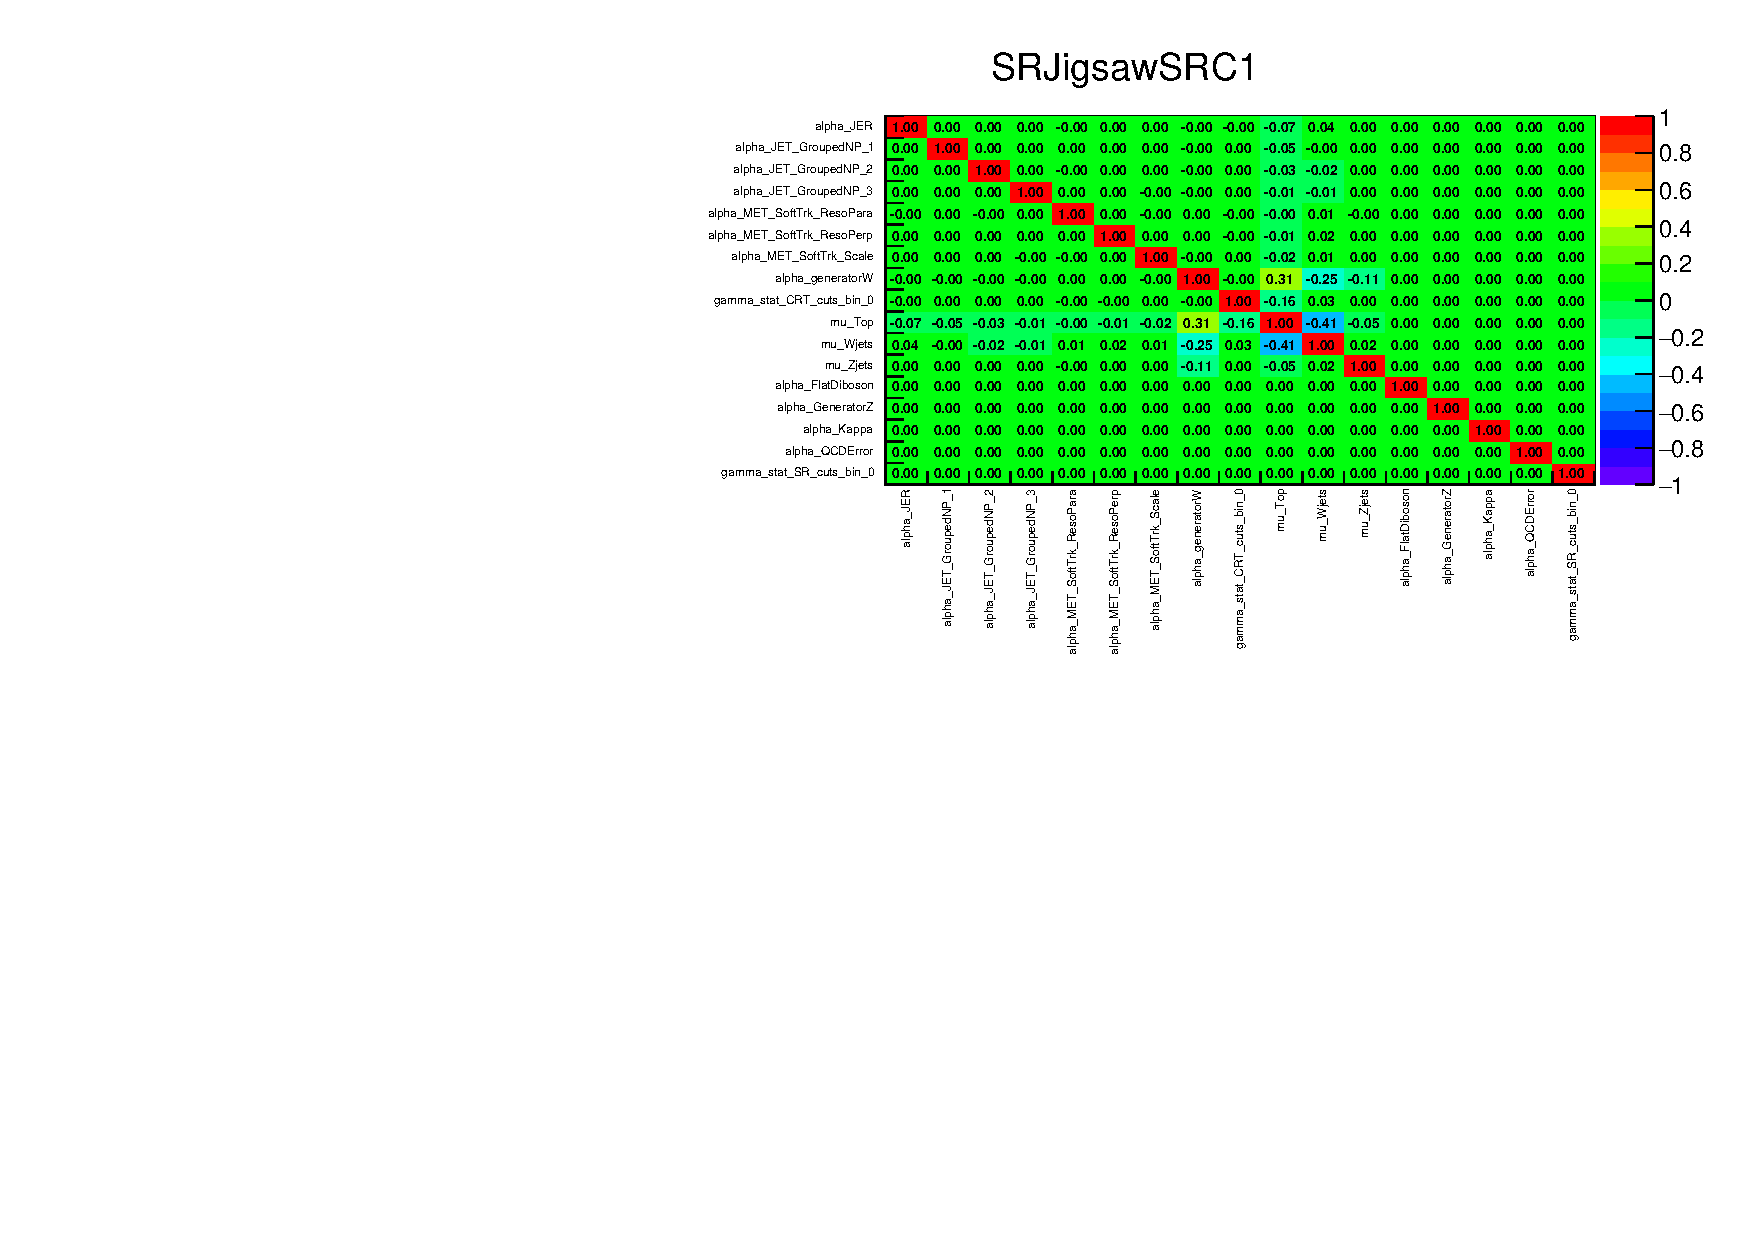
\includegraphics[width=.9\linewidth]{ATLAS-CONF-2016-078_INT/HistFitter/PullPlots/29_07_16/corr_SRJigsawSRC1}
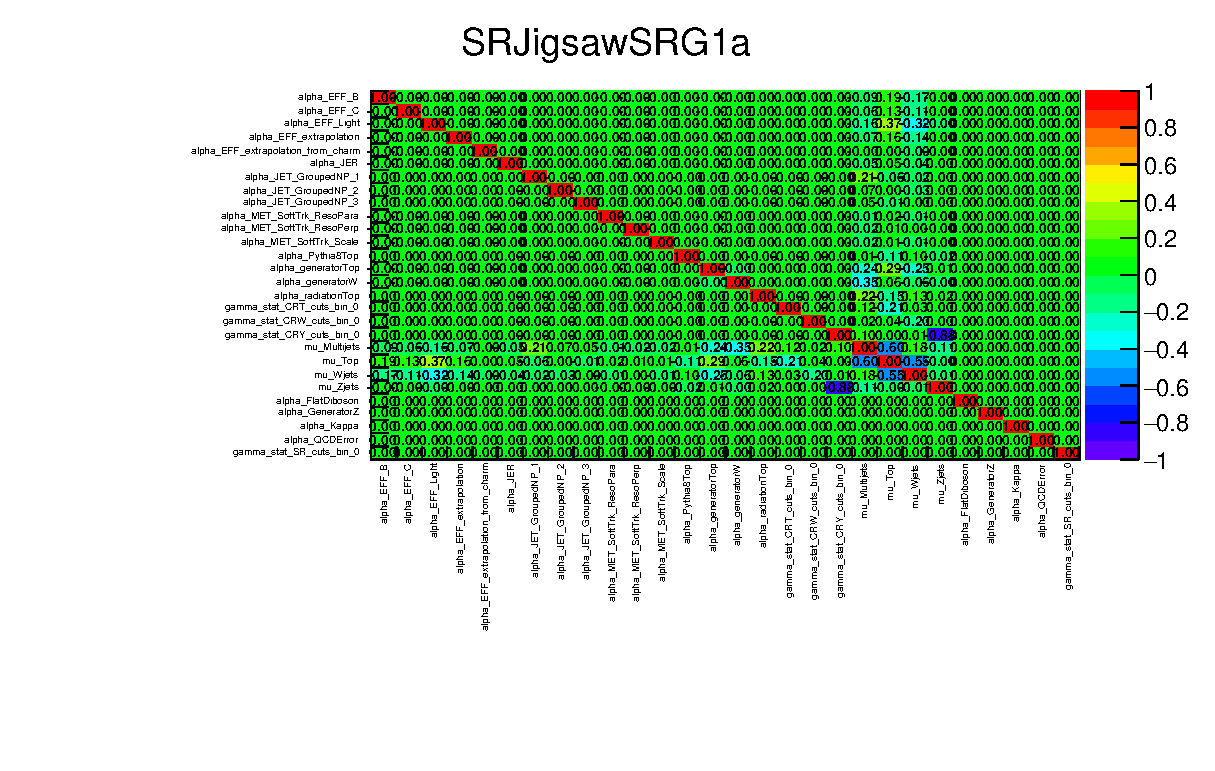
\includegraphics[width=.9\linewidth]{ATLAS-CONF-2016-078_INT/HistFitter/PullPlots/29_07_16/corr_SRJigsawSRG1a}
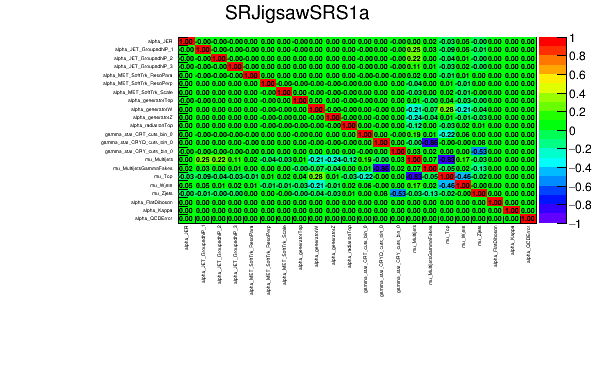
\includegraphics[width=.9\linewidth]{ATLAS-CONF-2016-078_INT/HistFitter/PullPlots/29_07_16/corr_SRJigsawSRS1a}
\end{figure}

%% This table is automatically generated from individual tables per signal region
%% you can update it via the script: ./makeAllSystTableInOne.py

\begin{table}[tbp]
%\small
\scriptsize
\begin{center}
%\begin{sidewaystable}
%\scriptsize
%\begin{center}
%\setlength{\tabcolsep}{0.0pc}
\begin{tabular}{|lrrrrrr|}
\hline
Channel  &  \textbf{ S1a } & \textbf{ S1b } & \textbf{ S2a } & \textbf{ S2b } & \textbf{ S3a } & \textbf{ S3b }  \\ \hline
Total bkg  &  $334$  &  $233$  &  $96$  &  $75$  &  $56$  &  $37$ \\
Total bkg unc.  &  $\pm 35$  [$10\%$]  &  $\pm 25$  [$11\%$]  &  $\pm 10$  [$10\%$]  &  $\pm 8$  [$11\%$]  &  $\pm 6$  [$11\%$]  &  $\pm 4$  [$11\%$] \\
\hline
MC statistics  &   --    &  $\pm 2.6$ [$1\%$]  &  $\pm 1.5$ [$2\%$]  &  $\pm 1.3$ [$2\%$]  &  $\pm 1.0$ [$2\%$]  &  $\pm 0.7$ [$2\%$] \\
$\Delta\mu_{Z,\mathrm{+jets}}$    &  $\pm 20$ [$6\%$]  &  $\pm 14$ [$6\%$]  &  $\pm 4$ [$4\%$]  &  $\pm 2.9$ [$4\%$]  &  $\pm 2.2$ [$4\%$]  &  $\pm 1.5$ [$4\%$] \\
$\Delta\mu_{W,\mathrm{+jets}}$    &  $\pm 10$ [$3\%$]  &  $\pm 7$ [$3\%$]  &  $\pm 3.1$ [$3\%$]  &  $\pm 2.3$ [$3\%$]  &  $\pm 1.6$ [$3\%$]  &  $\pm 1.1$ [$3\%$] \\
$\Delta\mu_{  \mathrm{ Top}}$       &  $\pm 6$ [$2\%$]  &  $\pm 4$ [$2\%$]  &  $\pm 1.5$ [$2\%$]  &  $\pm 1.1$ [$1\%$]  &  $\pm 0.9$ [$2\%$]  &  $\pm 0.6$ [$2\%$] \\
$\Delta\mu_{  \mathrm{ Multijet}}$  &  $\pm 0.09$ [$0\%$]  &  $\pm 0.05$ [$0\%$]  &  $\pm 0.02$ [$0\%$]  &   --    &   --    &   --   \\
CR$\gamma$ corr. factor  &  $\pm 12$ [$4\%$]  &  $\pm 8$ [$3\%$]  &  $\pm 4$ [$4\%$]  &  $\pm 2.9$ [$4\%$]  &  $\pm 2.2$ [$4\%$]  &  $\pm 1.4$ [$4\%$] \\
Theory Z  &  $\pm 23$ [$7\%$]  &  $\pm 16$ [$7\%$]  &  $\pm 7$ [$7\%$]  &  $\pm 6$ [$8\%$]  &  $\pm 4$ [$7\%$]  &  $\pm 2.8$ [$8\%$] \\
Theory W  &  $\pm 4$ [$1\%$]  &  $\pm 5$ [$2\%$]  &  $\pm 0.4$ [$0\%$]  &  $\pm 0.11$ [$0\%$]  &  $\pm 1.5$ [$3\%$]  &  $\pm 1.2$ [$3\%$] \\
Theory Top   &  $\pm 4$ [$1\%$]  &  $\pm 2.7$ [$1\%$]  &  $\pm 0.8$ [$1\%$]  &  $\pm 0.7$ [$1\%$]  &  $\pm 0.6$ [$1\%$]  &  $\pm 0.4$ [$1\%$] \\
Theory Diboson  &  $\pm 9$ [$3\%$]  &  $\pm 6$ [$3\%$]  &  $\pm 2.8$ [$3\%$]  &  $\pm 2.6$ [$3\%$]  &  $\pm 2.1$ [$4\%$]  &  $\pm 1.4$ [$4\%$] \\
Jet/MET   &  $\pm 3.3$ [$1\%$]  &  $\pm 1.5$ [$1\%$]  &  $\pm 0.6$ [$1\%$]  &  $\pm 0.6$ [$1\%$]  &  $\pm 1.2$ [$2\%$]  &  $\pm 1.0$ [$3\%$] \\
Multijet method  &  $\pm 0.7$ [$0\%$]  &  $\pm 0.4$ [$0\%$]  &  $\pm 0.08$ [$0\%$]  &   --    &   --    &   --   \\
\hline
\end{tabular}

\begin{tabular}{|lrrrrrr|}
\hline
Channel  &  \textbf{ G1a } & \textbf{ G1b } & \textbf{ G2a } & \textbf{ G2b } & \textbf{ G3a } & \textbf{ G3b }  \\ \hline
Total bkg  &  $40$  &  $18.8$  &  $27.8$  &  $8.5$  &  $5.8$  &  $1.7$ \\
Total bkg unc.  &  $\pm 4$  [$10\%$]  &  $\pm 2.5$  [$13\%$]  &  $\pm 3.4$  [$12\%$]  &  $\pm 1.4$  [$16\%$]  &  $\pm 1.1$  [$19\%$]  &  $\pm 0.4$  [$24\%$] \\
\hline
MC statistics  &  $\pm 1.6$ [$4\%$]  &  $\pm 1.0$ [$5\%$]  &  $\pm 1.2$ [$4\%$]  &  $\pm 0.6$ [$7\%$]  &  $\pm 0.4$ [$7\%$]  &  $\pm 0.23$ [$14\%$] \\
$\Delta\mu_{Z,\mathrm{+jets}}$  &  $\pm 1.5$ [$4\%$]  &  $\pm 0.7$ [$4\%$]  &  $\pm 1.6$ [$6\%$]  &  $\pm 0.5$ [$6\%$]  &  $\pm 0.4$ [$7\%$]  &  $\pm 0.1$ [$6\%$] \\
$\Delta\mu_{W,\mathrm{+jets}}$  &  $\pm 0.9$ [$2\%$]  &  $\pm 0.4$ [$2\%$]  &  $\pm 1.2$ [$4\%$]  &  $\pm 0.31$ [$4\%$]  &  $\pm 0.28$ [$5\%$]  &  $\pm 0.1$ [$6\%$] \\
$\Delta\mu_{\mathrm{ Top}}$  &  $\pm 0.8$ [$2\%$]  &  $\pm 0.33$ [$2\%$]  &  $\pm 0.9$ [$3\%$]  &  $\pm 0.23$ [$3\%$]  &  $\pm 0.07$ [$1\%$]  &  $\pm 0.1$ [$6\%$] \\
$\Delta\mu_{\mathrm{ Multijet}}$  &  $\pm 0.1$ [$0\%$]  &  --  &  $\pm 0.03$ [$0\%$]  &  $\pm 0.02$ [$0\%$]  &   --    &   --   \\
CR$\gamma$ corr. factor  &  $\pm 1.2$ [$3\%$]  &  $\pm 0.6$ [$3\%$]  &  $\pm 0.8$ [$3\%$]  &  $\pm 0.26$ [$3\%$]  &  $\pm 0.19$ [$3\%$]  &  $\pm 0.05$ [$3\%$] \\
Theory Z  &  $\pm 2.3$ [$6\%$]  &  $\pm 1.1$ [$6\%$]  &  $\pm 1.6$ [$6\%$]  &  $\pm 0.5$ [$6\%$]  &  $\pm 0.4$ [$7\%$]  &  $\pm 0.1$ [$6\%$] \\
Theory W  &  $\pm 1.1$ [$3\%$]  &  $\pm 1.3$ [$7\%$]  &  $\pm 0.3$ [$1\%$]  &  $\pm 0.7$ [$8\%$]  &  $\pm 0.6$ [$10\%$]  &  $\pm 0.16$ [$9\%$] \\
Theory Top   &  $\pm 1.2$ [$3\%$]  &  $\pm 0.7$ [$4\%$]  &  $\pm 1.0$ [$4\%$]  &  $\pm 0.4$ [$5\%$]  &  $\pm 0.4$ [$7\%$]  &  $\pm 0.26$ [$15\%$] \\
Theory Diboson  &  $\pm 1.3$ [$3\%$]  &  $\pm 0.8$ [$4\%$]  &  $\pm 1.5$ [$5\%$]  &  $\pm 0.6$ [$7\%$]  &  $\pm 0.31$ [$5\%$]  &  $\pm 0.13$ [$8\%$] \\
Jet/MET   &  $\pm 1.0$ [$3\%$]  &  $\pm 0.6$ [$3\%$]  &  $\pm 0.4$ [$1\%$]  &  $\pm 0.17$ [$2\%$]  &  $\pm 0.22$ [$4\%$]  &  $\pm 0.05$ [$3\%$] \\
Multijet method  &  $\pm 0.24$ [$1\%$]  &  $\pm 0.12$ [$1\%$]  &  $\pm 0.5$ [$2\%$]  &  $\pm 0.4$ [$5\%$]  &   --    &   --   \\
\hline
\end{tabular}

\begin{tabular}{|lrrrrr|}
\hline
Channel                           & \textbf{ C1 }   & \textbf{ C2 }  & \textbf{ C3 }  & \textbf{ C4 }   & \textbf{ C5 }   \\ \hline
Total bkg                         & $14.5$              & $59$               & $110$              & $10.5$              & $7.3$               \\
Total bkg unc.                    & $\pm 2.2$  [$15\%$] & $\pm 6$  [$10\%$]  & $\pm 11$  [$10\%$] & $\pm 1.5$  [$14\%$] & $\pm 1.4$  [$19\%$] \\
\hline
MC statistics                     & $\pm 0.7$ [$5\%$]   & $\pm 1.7$ [$3\%$]  & $\pm 2.4$ [$2\%$]  & $\pm 0.6$ [$6\%$]   & $\pm 0.6$ [$8\%$]   \\
$\Delta\mu_{Z,\mathrm{+jets}}$    & $\pm 0.5$ [$3\%$]   & $\pm 1.9$ [$3\%$]  & $\pm 2.5$ [$2\%$]  & $\pm 0.31$ [$3\%$]  & $\pm 0.13$ [$2\%$]  \\
$\Delta\mu_{W,\mathrm{+jets}}$    & $\pm 0.4$ [$3\%$]   & $\pm 1.7$ [$3\%$]  & $\pm 5$ [$5\%$]    & $\pm 0.4$ [$4\%$]   & $\pm 0.25$ [$3\%$]  \\
$\Delta\mu_{\mathrm{ Top}}$       & $\pm 0.33$ [$2\%$]  & $\pm 1.3$ [$2\%$]  & $\pm 4$ [$4\%$]    & $\pm 0.31$ [$3\%$]  & $\pm 0.4$ [$5\%$]   \\
$\Delta\mu_{\mathrm{ Multijet}}m$ & --                  & $\pm 0.1$ [$0\%$]  & $\pm 0.06$ [$0\%$] & --                  & $\pm 0.1$ [$1\%$]   \\
CR$\gamma$ corr. factor $\kappa$  & $\pm 0.5$ [$3\%$]   & $\pm 1.8$ [$3\%$]  & $\pm 2.3$ [$2\%$]  & $\pm 0.29$ [$3\%$]  & $\pm 0.13$ [$2\%$]  \\
Theory Z                          & $\pm 0.8$ [$6\%$]   & $\pm 3.5$ [$6\%$]  & $\pm 4$ [$4\%$]    & $\pm 0.6$ [$6\%$]   & $\pm 0.24$ [$3\%$]  \\
Theory W                          & $\pm 1.3$ [$9\%$]   & $\pm 0.03$ [$0\%$] & $\pm 2.0$ [$2\%$]  & $\pm 1.0$ [$10\%$]  & $\pm 0.13$ [$2\%$]  \\
Theory Top                        & $\pm 0.5$ [$3\%$]   & $\pm 1.3$ [$2\%$]  & $\pm 3.2$ [$3\%$]  & $\pm 0.6$ [$6\%$]   & $\pm 0.9$ [$12\%$]  \\
Theory Diboson                    & $\pm 1.0$ [$7\%$]   & $\pm 4$ [$7\%$]    & $\pm 6$ [$5\%$]    & $\pm 0.27$ [$3\%$]  & $\pm 0.4$ [$5\%$]   \\
Jet/MET                           & $\pm 0.5$ [$3\%$]   & $\pm 1.5$ [$3\%$]  & $\pm 3.1$ [$3\%$]  & $\pm 0.24$ [$2\%$]  & $\pm 0.5$ [$7\%$]   \\
Multijet method                   & $\pm 0.09$ [$1\%$]  & $\pm 0.4$ [$1\%$]  & $\pm 2.1$ [$2\%$]  & --                  & $\pm 0.18$ [$2\%$]  \\
\hline
\end{tabular}

%\end{tabular*}
\end{center}
\caption{
Breakdown of the dominant systematic uncertainties in the background estimates.
The individual uncertainties can be correlated, and do not necessarily add in quadrature.
$\Delta_{\mu}$ uncertainties result from control region statistical uncertainties and the systematic uncertainties in the appropriate control region.
In brackets, uncertainties are given relative to the expected total background yield, also presented in the Table. Empty cells (indicated by a `-') correspond to uncertainties $<$0.1\%. \label{tab:BreakdownSysSRCompressed_RJR}}
%\end{sidewaystable}
\end{table}


\section{Exclusion plots}


\begin{figure}[tbph]
\begin{center}
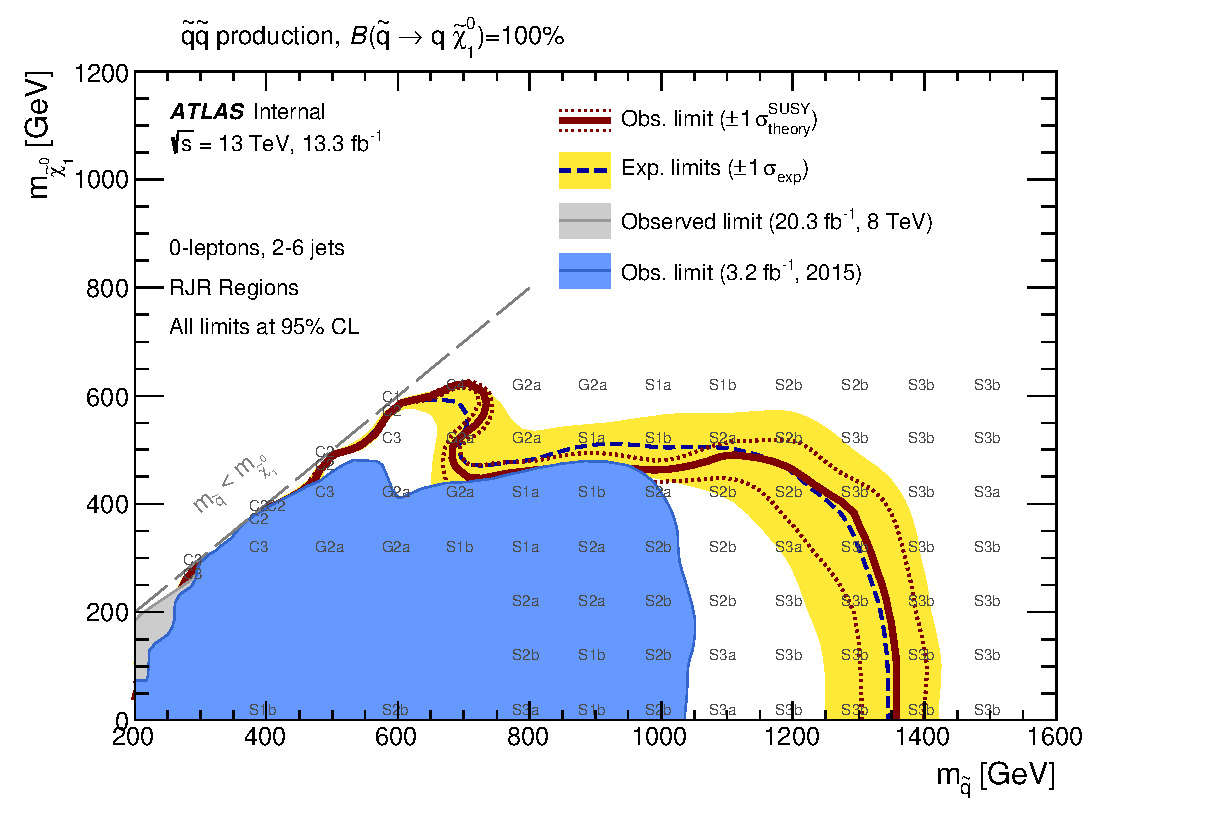
\includegraphics[width=0.45\textwidth]{figures/ATLAS-CONF-2016-078_INT/Sensitivity/RJR/atlasCLs_SS_direct_showSR}
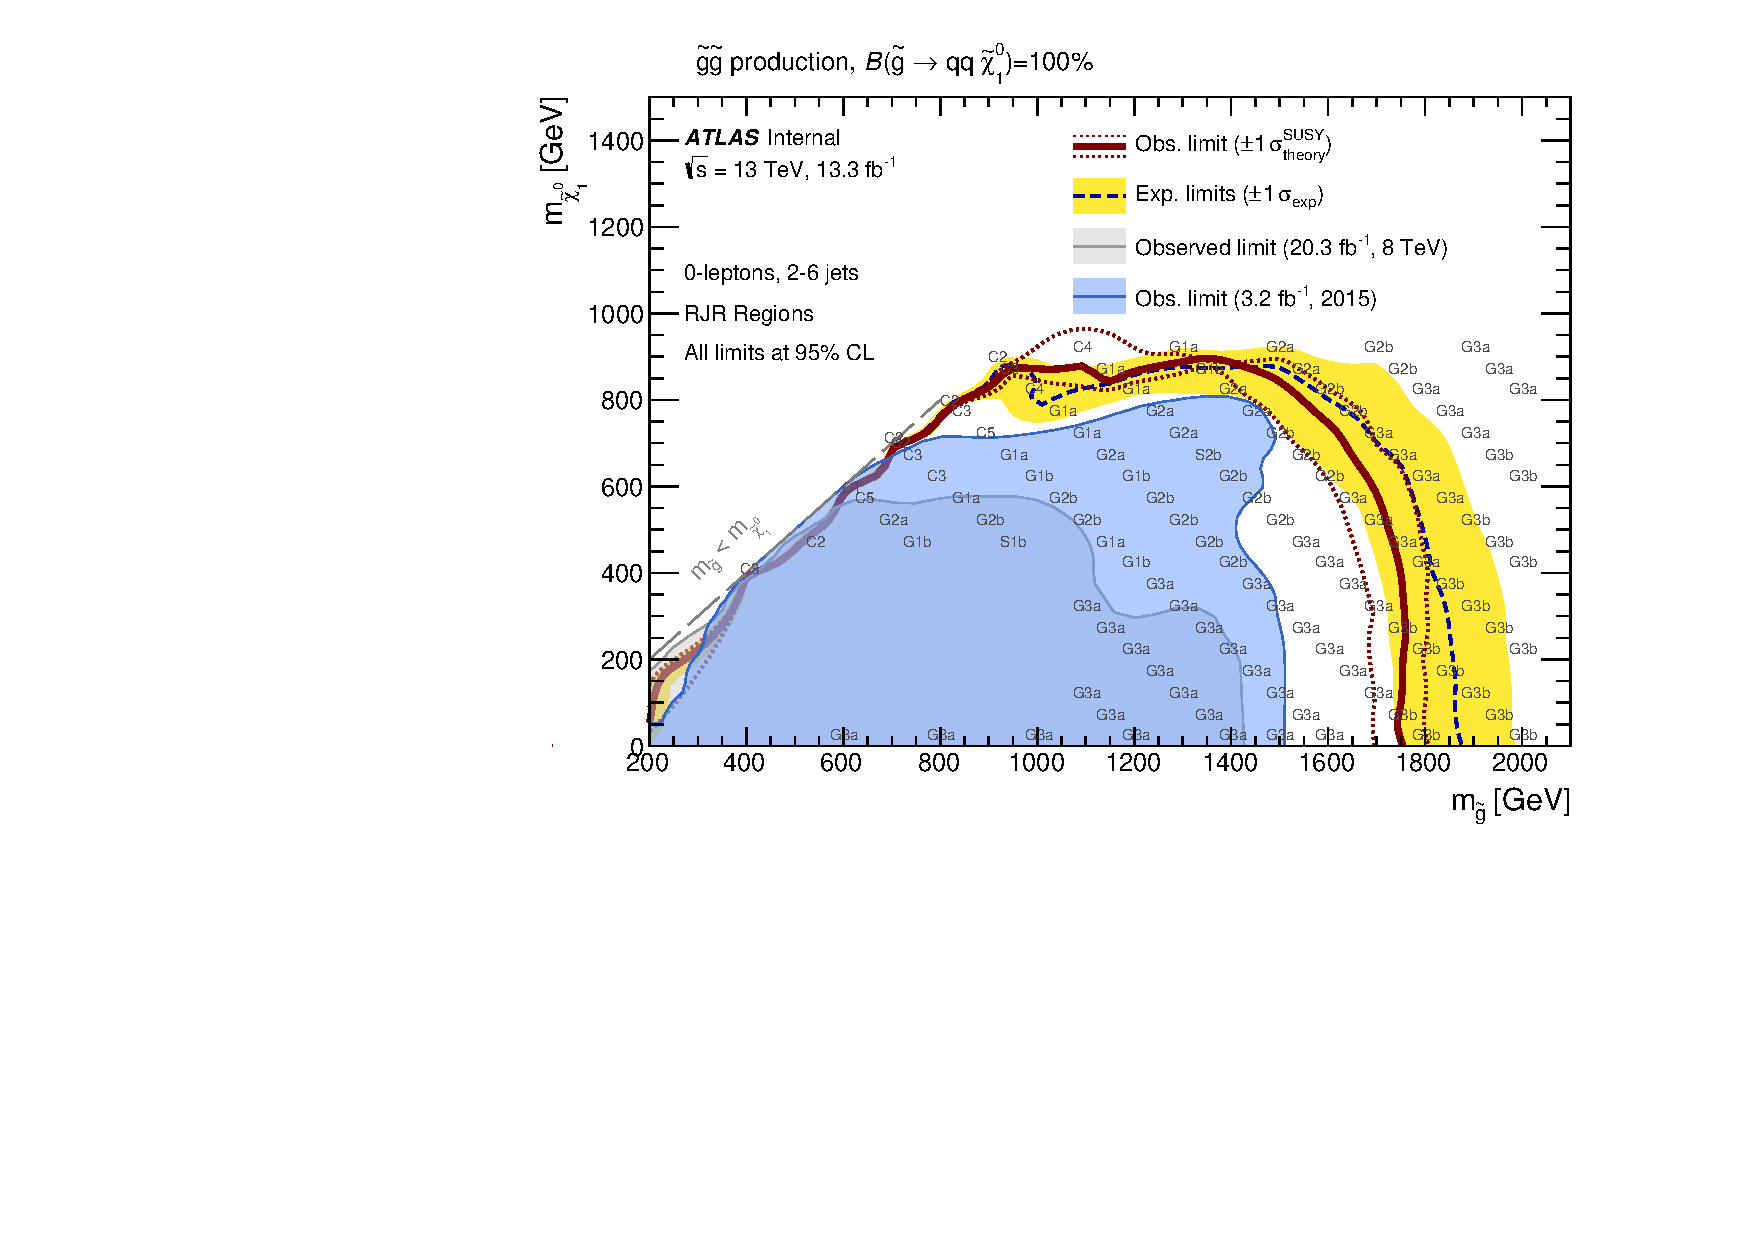
\includegraphics[width=0.45\textwidth]{figures/ATLAS-CONF-2016-078_INT/Sensitivity/RJR/atlasCLs_GG_direct_showSR}
\end{center}
\caption{Exclusion limits for direct production of (a) light-flavour squark pairs with decoupled gluinos and (b) gluino pairs with decoupled squarks.
Gluinos (light-flavour squarks) are required to decay to two quarks (one quark) and a neutralino LSP.
Exclusion limits are obtained by using the signal region with the best expected sensitivity at each point.
The blue dashed lines show the expected limits at 95\% CL, with the light (yellow) bands indicating the $1\sigma$ excursions due to experimental and background-only  theoretical uncertainties.
Observed limits are indicated by medium dark (maroon) curves where the solid contour represents the nominal limit, and the dotted lines are obtained by varying the signal cross-section by the renormalization and factorization scale and PDF uncertainties.
Results are compared with the observed limits obtained by the previous ATLAS searches with no leptons, jets and missing transverse momentum~\cite{0-leptonPaper,0LPaper_13TeV}.}
\label{fig:sensitivitytext}
\end{figure}
